%----------------------------------------------------------------------------------------
%	Capítulo 5
%----------------------------------------------------------------------------------------

\pagestyle{myportland}
%\pagenumbering{arabic}
\doublespacing
\chapter[----- Diseño mecatrónico integral]{Diseño mecatrónico integral}
\thispagestyle{myportland}

%%%%%%%%%%%%%%%%%%%%%%%%%%%%%%%%%%%%%%%%%%%%%%%%%%%%%%%%%%%%%%
%%%%%                                                    %%%%%
%%%%%             DISEÑO MECATRÓNICO EN SÍ               %%%%%
%%%%%                                                    %%%%%
%%%%%%%%%%%%%%%%%%%%%%%%%%%%%%%%%%%%%%%%%%%%%%%%%%%%%%%%%%%%%%

%% NUEVA SECCIÓN X.X
\section{Desarrollo de diseño mecatrónico integral}

En la sección llamada \textit{"Desarrollo del diseño mecatrónico conceptual"} \footnote{\cite{DiazVergara2020}} se analizó el concepto de solución óptimo. En la Figura \ref{fig:estado diseno mecatronico etapa 3} se muestra la etapa final de unir las sub-soluciones para desarrollar una forma viable de implementarlos de una forma integral.

\begin{myfigure}[H]
	\centering
	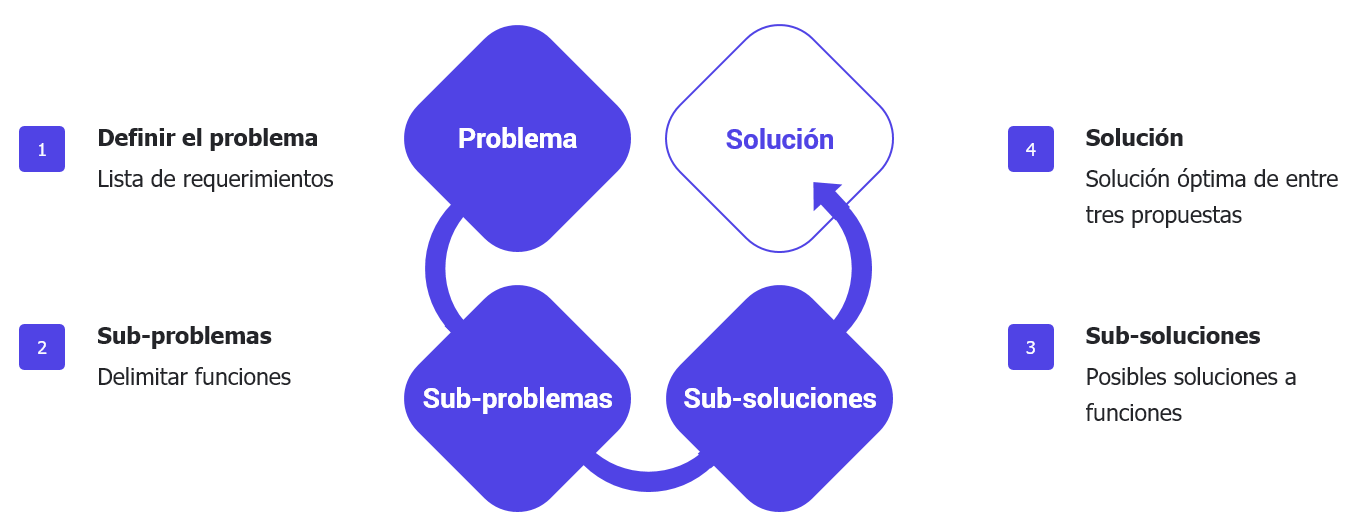
\includegraphics[width=1\textwidth]{chapter5/estado diseno subsoluciones.png}
	\caption{Estado de diseño mecatrónico: sub-soluciones}
	\begin{myflushleftportland}
		Fuente: Elaboración propia
	\end{myflushleftportland}
	\label{fig:estado diseno mecatronico etapa 3}
\end{myfigure}

Según el proceso de diseño indicado en la norma VDI 2221 que se muestra en la Figura \ref{fig:vdi2221} se parte del diseño conceptual propuesto (5) y se presenta el diseño integral (6)\footnote{\cite{Pahl2007}}, también llamado diseño de ingeniería, que abarca diferentes puntos: dimensionamiento del sistema; cálculos; selección técnica de materiales entorno a su aplicación; selección técnica de sensores; actuadores y dispositivos de control; lógica del control del sistema y su estrategia; planos mecánicos: ensamble y despiece; planos eléctricos y/o electrónicos; simulaciones de la máquina y una estimación de costos.

\begin{myfigure}[H]
	\centering
	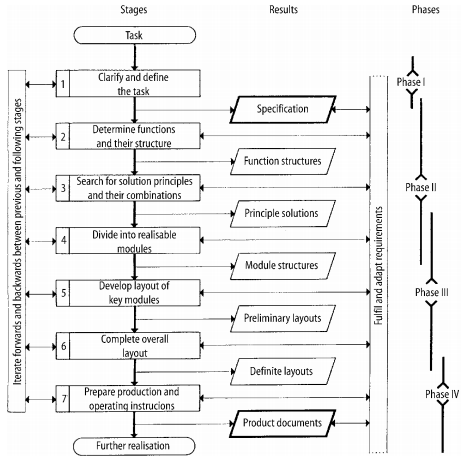
\includegraphics[width=0.75\textwidth]{chapter5/vdi2221.png}
	\caption{Fases de diseño según VDI 2221}
	\begin{myflushleftportland}
		Fuente: \cite{Pahl2007}
	\end{myflushleftportland}
	\label{fig:vdi2221}
\end{myfigure}



%% NUEVA SECCIÓN X.X.X
\subsection{Descripción del sistema integral}
\label{ssec:descripcion del sistema integral}

La máquina clasificadora y contadora de truchas\footnote{CCT}, y su sistema respectivo tienen como función principal recepcionar truchas mediante una tolva, procesar la clasificación, conteo y distribución hacia tres jaulas flotantes en medio de la Laguna de Paucarcocha.\footnote{\cite{DiazVergara2020}} La máquina se sitúa sobre el agua y es empleada por un operario, que se encarga de extraer truchas con una sacadera telescópica\footnote{También llamada cal-cal.}.

\textcolor{blue}{[BORRADOR] Terminar de explicar la descripción [/BORRADOR]}\\

En las siguientes páginas se analizan diversos puntos generales concernientes al sistema: arquitectura de hardware, la selección de materiales de fabricación, la selección de materiales de fabricación.


%% NUEVO SUBSECCION X.X.X.X
\subsubsection{Arquitectura de hardware}

En la Figura \ref{fig:arquitectura de hardware del sistema} se muestra la propuesta de arquitectura de hardware. Esta arquitectura nos muestra las entradas de energía del sistema, su redistribución a cada componente, el control asociado a cada pieza mediante el subsistema de control y los protocolos o energía asociado a cada par de bloques. Además, el tipo de conexión se detalla en la leyenda.

\begin{myfigure}[H]
	\centering
	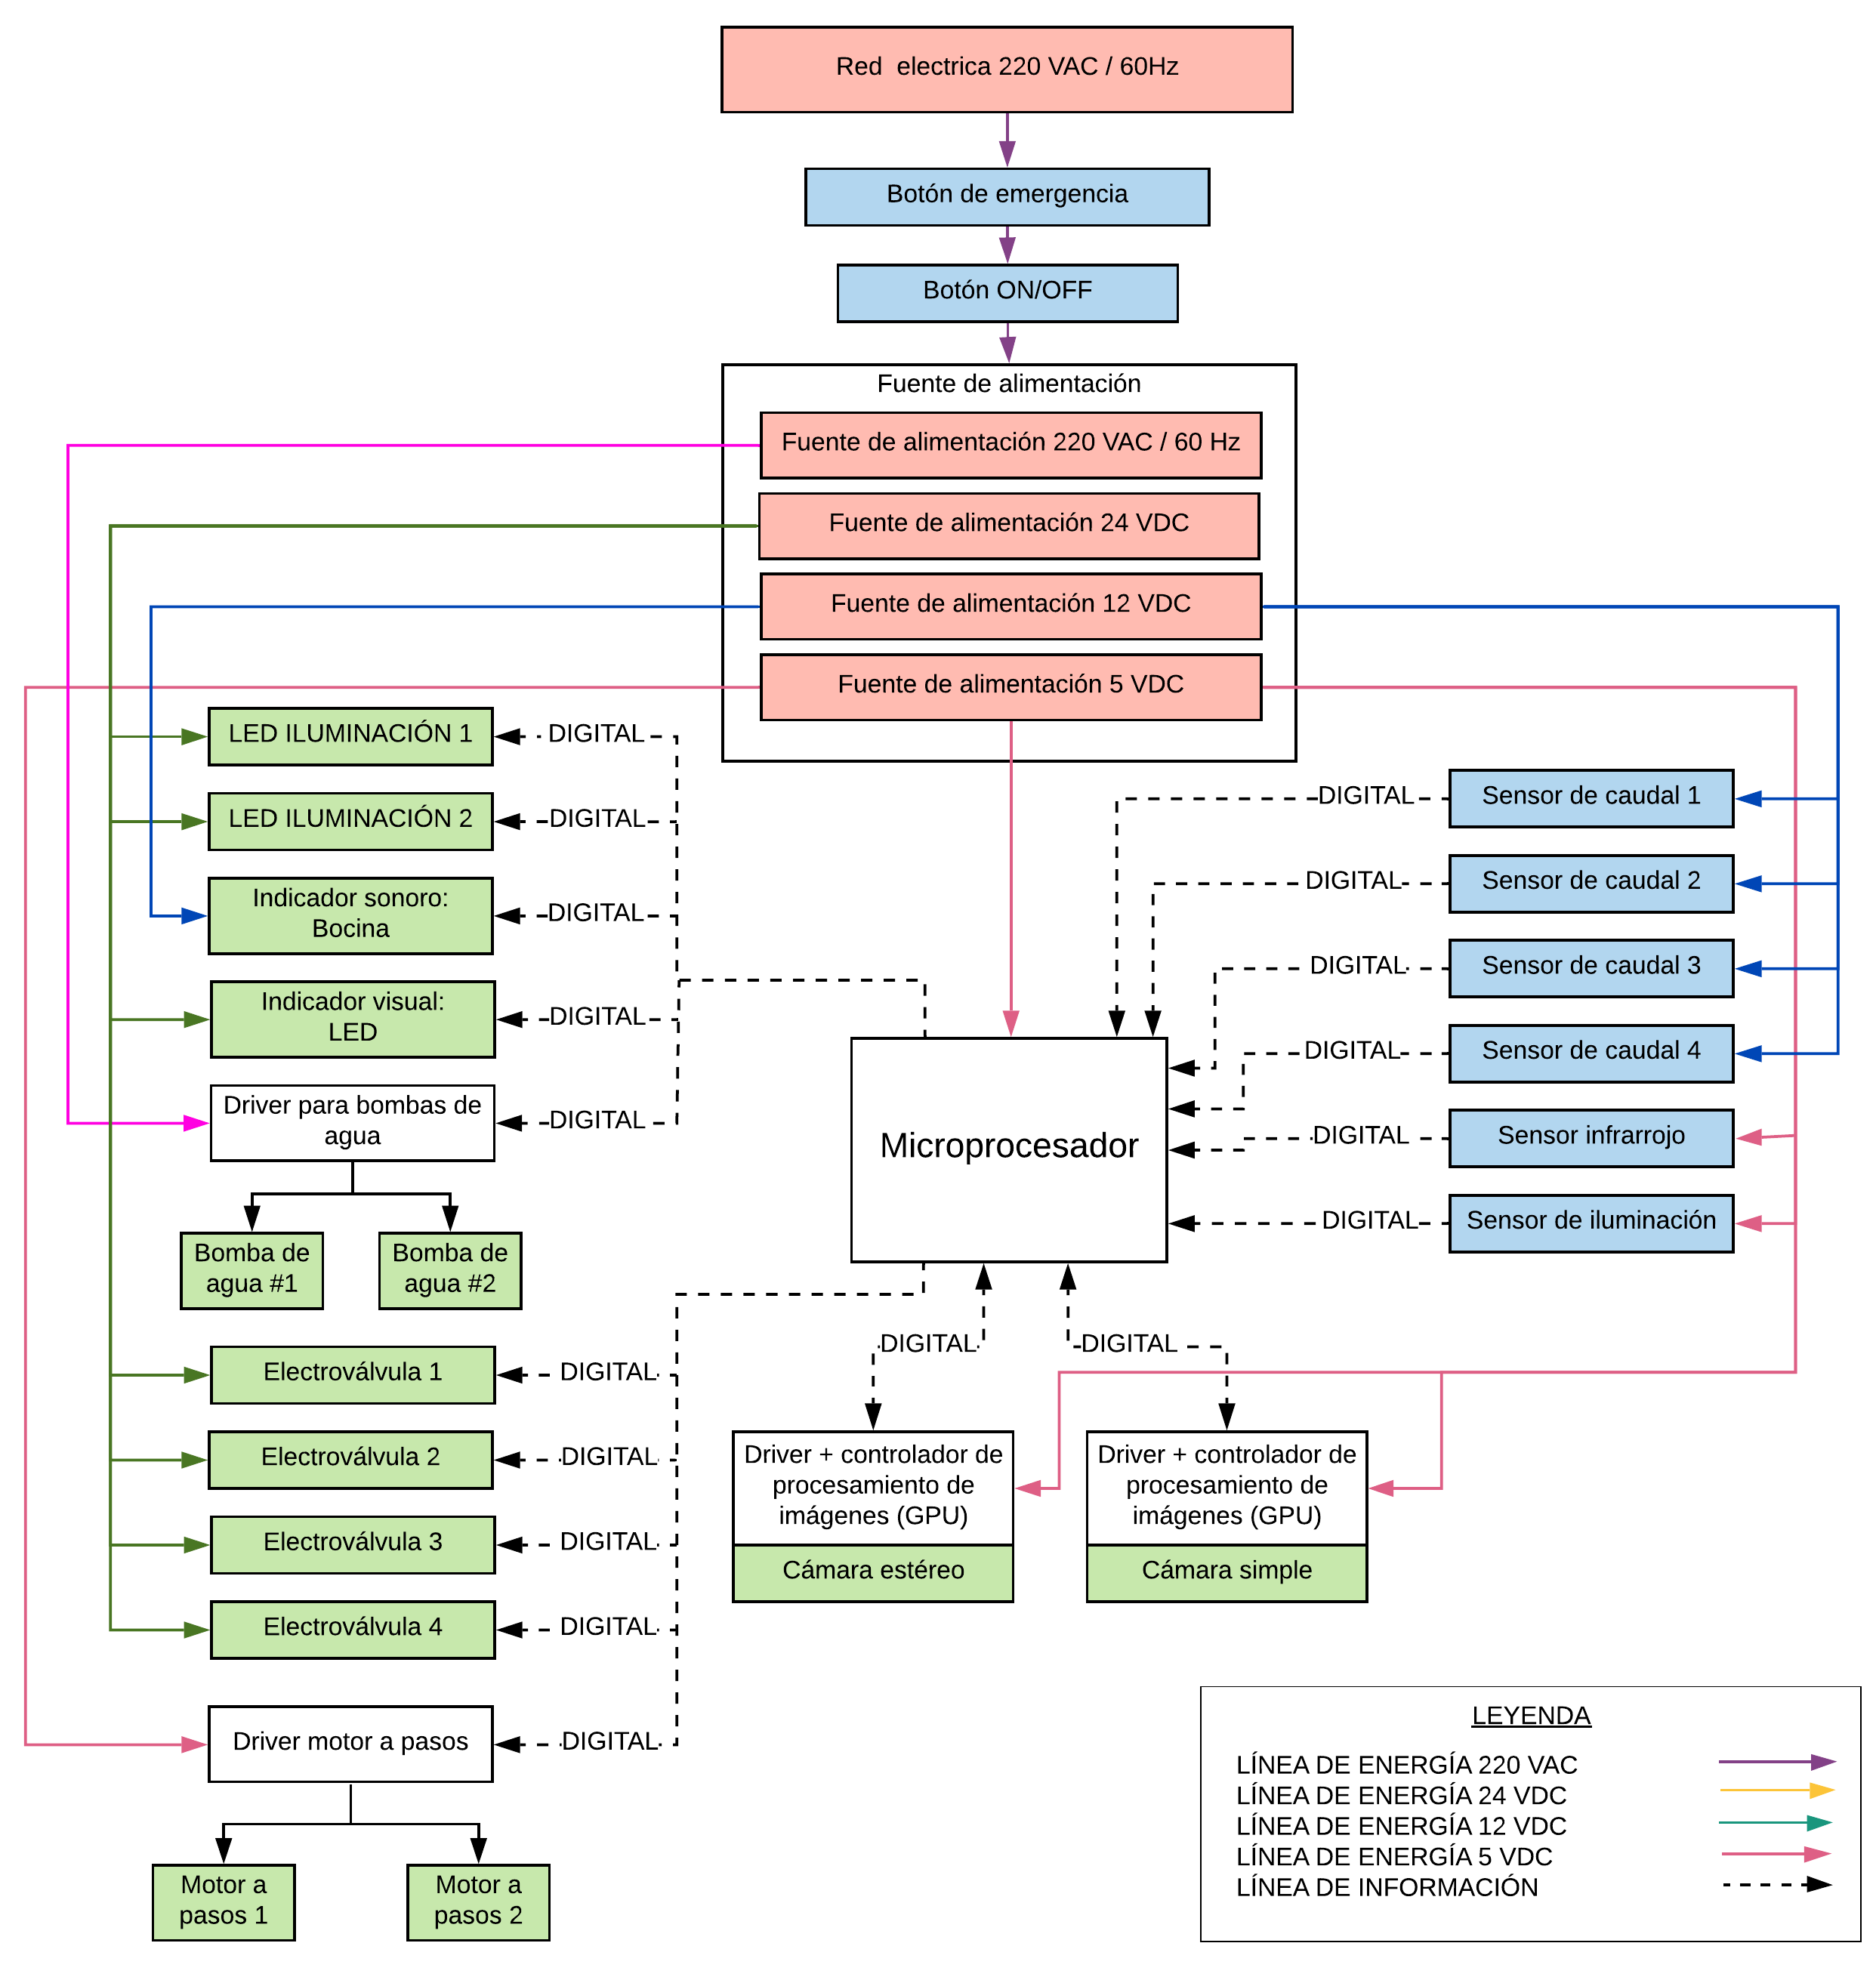
\includegraphics[width=0.75\textwidth]{chapter5/arquitectura de hardware del sistema.png}
	\caption{Arquitectura de hardware del sistema}
	\begin{myflushleftportland}
		Fuente: Elaboración propia.
	\end{myflushleftportland}
	\label{fig:arquitectura de hardware del sistema}
\end{myfigure}


%% NUEVO SUBSECCION X.X.X.X
\subsubsection{Selección de materiales de fabricación}
\label{sssec:seleccion de materiales de fabricacion}

Cada subsistema posee mecanismos que se rigen por un material en general, esto incluye a las partes principales del subsistema. Sin embargo, no considera el material de tornillos, ajustes o dispositivos similares. Existen así mismos requisitos que se pueden generalizar para todos los subsistemas por el entorno de trabajo a la que estará sometida la máquina detallados en la \textit{"Lista de requerimientos"} \footnote{\cite{DiazVergara2020}.}. Basado en dichas demandas, cada subsistema es analizado y presentado con dos alternativas posibles de materiales. Consecuentemente, se elige un material decisivo para ser empleado bajo el sustento técnico que se explicará en los siguientes párrafos.

\begin{itemize}
	\item \textbf{Subsistema de recepción y traslado de truchas:} Cuenta con dos mecanismos; recepción de truchas y tuberías de traslado. El primero debe recepcionar a las truchas y dirigirlas al mecanismo de tuberías. El segundo debe trasladar a las truchas de un punto a otro de la máquina mediante las tuberías. En la Tabla \ref{tab:tabla comparativa de propiedades entre aluminio vs acero inoxidable} se comparan técnicamente las propiedades de dos materiales posibles.
	
	\begin{mytable}[H]
		\centering
		\caption{Tabla comparativa de propiedades entre $Aluminio$ vs $Acero \quad Inoxidable$}
		\label{tab:tabla comparativa de propiedades entre aluminio vs acero inoxidable}
		\begin{tabular}{|l|c|c|}
			\hline
			\multicolumn{1}{|c|}{\textbf{Propiedad}} & \textbf{Aluminio} & \textbf{Acero Inoxidable} \\ \hline
			Módulo de Young ($GPa$) & 69 & 200 \\ \hline
			Esfuerzo de fatiga $Y$ ($MPa$) & 58-110 & 210-440 \\ \hline
			Resistencia a la tracción ($MPa$) & 130-410 & 580-1180 \\ \hline
			Temperatura máxima mecánica (°$C$) & 650 & 1450 \\ \hline
			Conductividad térmica ($W/m-K$) & 170 & 16 \\ \hline
			Expansión térmica (${\mu}m/m-K$) & 24 & 17 \\ \hline
			Conductividad eléctrica ($\%$) & 43 & 2.4 \\ \hline
			Densidad ($g/cm^3$) & 2.7 & 7.8 \\ \hline
		\end{tabular}
		\begin{flushleft}
			*Terminología técnica de los materiales: Aluminio 6061, Acero Inoxidable ANSI 304.\\		
			Fuente: \cite{MakeItFrom2020}.
		\end{flushleft}
	\end{mytable}

	\textcolor{blue}{[BORRADOR] Se elige el material Aluminio 6061 por la alta durabilidad, ... EXPLICAR LA SELECCIÓN DE ALUMINIO [/BORRADOR]} 
	
	\item \textbf{Subsistema de procesamiento de imágenes:} Cuenta con dos mecanismos; tuberías y juego de espejos. El primero debe brindar a la cámara suficiente transparencia para obtener una fotografía adecuada. El segundo debe brindar a la cámara más perfiles del cuerpo que es trasladado por la tubería. En la Tabla \ref{tab:tabla comparativa de propiedades entre pmma vs pvdf} se compara técnicamente las propiedades de dos materiales posibles.
	
	\begin{mytable}[H]
		\centering
		\caption{Tabla comparativa de propiedades entre $PMMA$ vs $PVDF$}
		\label{tab:tabla comparativa de propiedades entre pmma vs pvdf}
		\begin{tabular}{|l|c|c|}
			\hline
			\multicolumn{1}{|c|}{\textbf{Propiedad}} & \multicolumn{1}{c|}{\textbf{PMMA}} & \textbf{PVDF} \\ \hline
			Resistencia al impacto: con muescas ($J/m$) & 74     & 180   \\ \hline
			Expansión térmica (${\mu}m/m-K$)  & 76 & 120 \\ \hline
			Densidad ($g/cm^3$) & 1.2 & 1.8  \\ \hline
			Resistencia al peso  & 32 & 20 \\ \hline
			Alargamiento a la rotura ($ \% $) & 4 & 49 \\ \hline
			Incidencia de luz trasmitida ($ \% $) & 92 & - \\ \hline
			Índice de refracción & 1.5 & 1.4 \\ \hline			
		\end{tabular}
		\begin{flushleft}
			*Terminología técnica de los materiales: Polimetilmetacrilato (Acrílico)(PMMA), Fluoruro de polivinilideno (PVDF).\\		
			Fuente: \cite{Brydson1999,Berins1991,Harper2000,MakeItFrom2020}.
		\end{flushleft}
	\end{mytable}

	\textcolor{blue}{[BORRADOR] Se elige el material ... por .... EXPLICAR LA SELECCIÓN [/BORRADOR] Comparar entre HDPE y otros termoplásticos.} 
	
	\item \textbf{Subsistema de procesamiento de suministro de energía:} Los materiales son propios de los dispositivos que serán adquiridos.
	
	\item \textbf{Subsistema de control e interacción con el usuario:} Los materiales son propios de los dispositivos que serán adquiridos.
	
	\item \textbf{Subsistema de flotación:} Cuenta con dos mecanismos; armadura y flotadores. El primero debe funcionar como esqueleto para los otros subsistemas y del mismo. El segundo debe mantener el sistema a flote.
	
	\textcolor{blue}{[BORRADOR] Presentar la Tabla siguiente [/BORRADOR]} 
	
	\begin{mytable}[H]
		\centering
		\caption{Tabla comparativa de propiedades entre $HDPE$ vs $PVC-U$}
		\label{tab:tabla comparativa de propiedades entre hdpe vs pvcu}
		\begin{tabular}{|l|c|c|}
			\hline
			\multicolumn{1}{|c|}{\textbf{Propiedad}} & \textbf{HDPE} & \textbf{PVC-U} \\ \hline
			Densidad ($g/cm^3$) & 1.0-1.3 & 1.4 \\ \hline
			Elongación a rotura ($\%$) & 2.5-100 & 58 \\ \hline
			Resistencia al impacto ($J/m$) & 50-260 & 360 \\ \hline
			Resistencia al peso: Flexión & 19-32 & 20 \\ \hline
			Resistencia a la tracción ($MPa$) & 24-80 & 47 \\ \hline
		\end{tabular}
		\begin{flushleft}
			*Terminología técnica de los materiales: Polietileno de alta densidad (HDPE), Cloruro de polivinilo no plastificado (rígido) (uPVC, PVC-U)\\		
			Fuente: \cite{Brydson1999,Berins1991,Harper2000,MakeItFrom2020}.
		\end{flushleft}
	\end{mytable}
	
	\textcolor{blue}{[BORRADOR] Se elige el material ... por .... EXPLICAR LA SELECCIÓN [/BORRADOR] Comparar entre HDPE y otros termoplásticos.} 
	
\end{itemize}

En las Tablas \ref{tab:tabla comparativa de propiedades entre aluminio vs acero inoxidable}, \ref{tab:tabla comparativa de propiedades entre pmma vs pvdf} y \ref{tab:tabla comparativa de propiedades entre hdpe vs pvcu} se comparan diversos materiales para el correspondiente subsistema. Los materiales de fabricación finales para cada subsistema se muestran en la Tabla \ref{tab:materiales de fabricacion por subsistema}, fueron seleccionados por su superioridad en las propiedades técnicas que son valoradas en este proyecto. 

\begin{savenotes}
\begin{mytable}[H]
	\centering
	\caption{Materiales de fabricación por subsistema}
	\label{tab:materiales de fabricacion por subsistema}
	\begin{tabular}{|l|c|c|}
		\hline
		\multicolumn{1}{|c|}{\textbf{Subsistema}} & \multicolumn{1}{c|}{\textbf{Mecanismo}} & \textbf{Material} \\ \hline
		Recepción y traslado de truchas      & Recepción de truchas   & Acero Inoxidable            \\ \hline
		Recepción y traslado de truchas      & Tuberías de traslado   & PVC-U                         \\ \hline
		Procesamiento de imágenes            & Tubería                & PMMA  \\ \hline
		Procesamiento de imágenes            & Juego de espejos       & PMMA  \\ \hline
		Suministro de energía                & \multicolumn{1}{c|}{-} & -                           \\ \hline
		Control e interacción con el usuario & \multicolumn{1}{c|}{-} & -                           \\ \hline
		Flotación                            & Armadura               & Aluminio o Acero Inoxidable \\ \hline
		Flotación                            & Flotadores             & HDPE                         \\ \hline
	\end{tabular}
	\begin{flushleft}
	*Terminología técnica de los materiales: Cloruro de polivinilo no plastificado (Rígido) (uPVC, PVC-U), Polimetilmetacrilato ISO 24026-1:2020\footnote{\href{https://www.iso.org/standard/77547.html}{Estándar ISO detallado}. Antecesor: 8257-1:1998. Estándar ASTM: D788-96} (Acrílico) (PMMA), Polietileno de alta densidad (HDPE), Acero Inoxidable 304, Aluminio 6061 (AL), Fluoruro de polivinilideno (PVDF).\\	
	Fuente: Elaboración propia.
	\end{flushleft}
\end{mytable}
\end{savenotes}

%% NUEVA SECCIÓN X.X.X
\subsection{Subsistema de recepción y traslado de truchas}
\label{ssec:subsistema de recepcion y traslado de truchas}

Este subsistema consiste en encapsular los mecanismos físicos que están en el ciclo que sigue una trucha dentro de la máquina: tolva, tuberías, bomba de agua, distribución física por mecanismos, caudales apropiados y el control respectivo. Los puntos mencionados se detallan en las siguientes páginas.

%% NUEVO SUBSECCION X.X.X.X
\subsubsection{Diseño de tolva de recepción de truchas}

El diseño implica un análisis sobre las situaciones que suceden cuando se realiza el proceso de depositar las truchas. En la Figura \ref{fig:calculo de dimensiones y angulo de la tolva} se analiza dicha situación con la finalidad de escoger un ángulo de elevación de la tolva ($\beta$) adecuado. Respecto a la tolva, se designan los siguientes valores iniciales: $A_{min},B_{min}=200 mm.$; $\beta \in [0;45] ^\circ$; ${tolva}=150 mm.$. Además, debe cumplirse que $A_{max}>B_{max}$ orientado hacia el operario que depositará la trucha.

\begin{myfigure}[H]
	\centering
	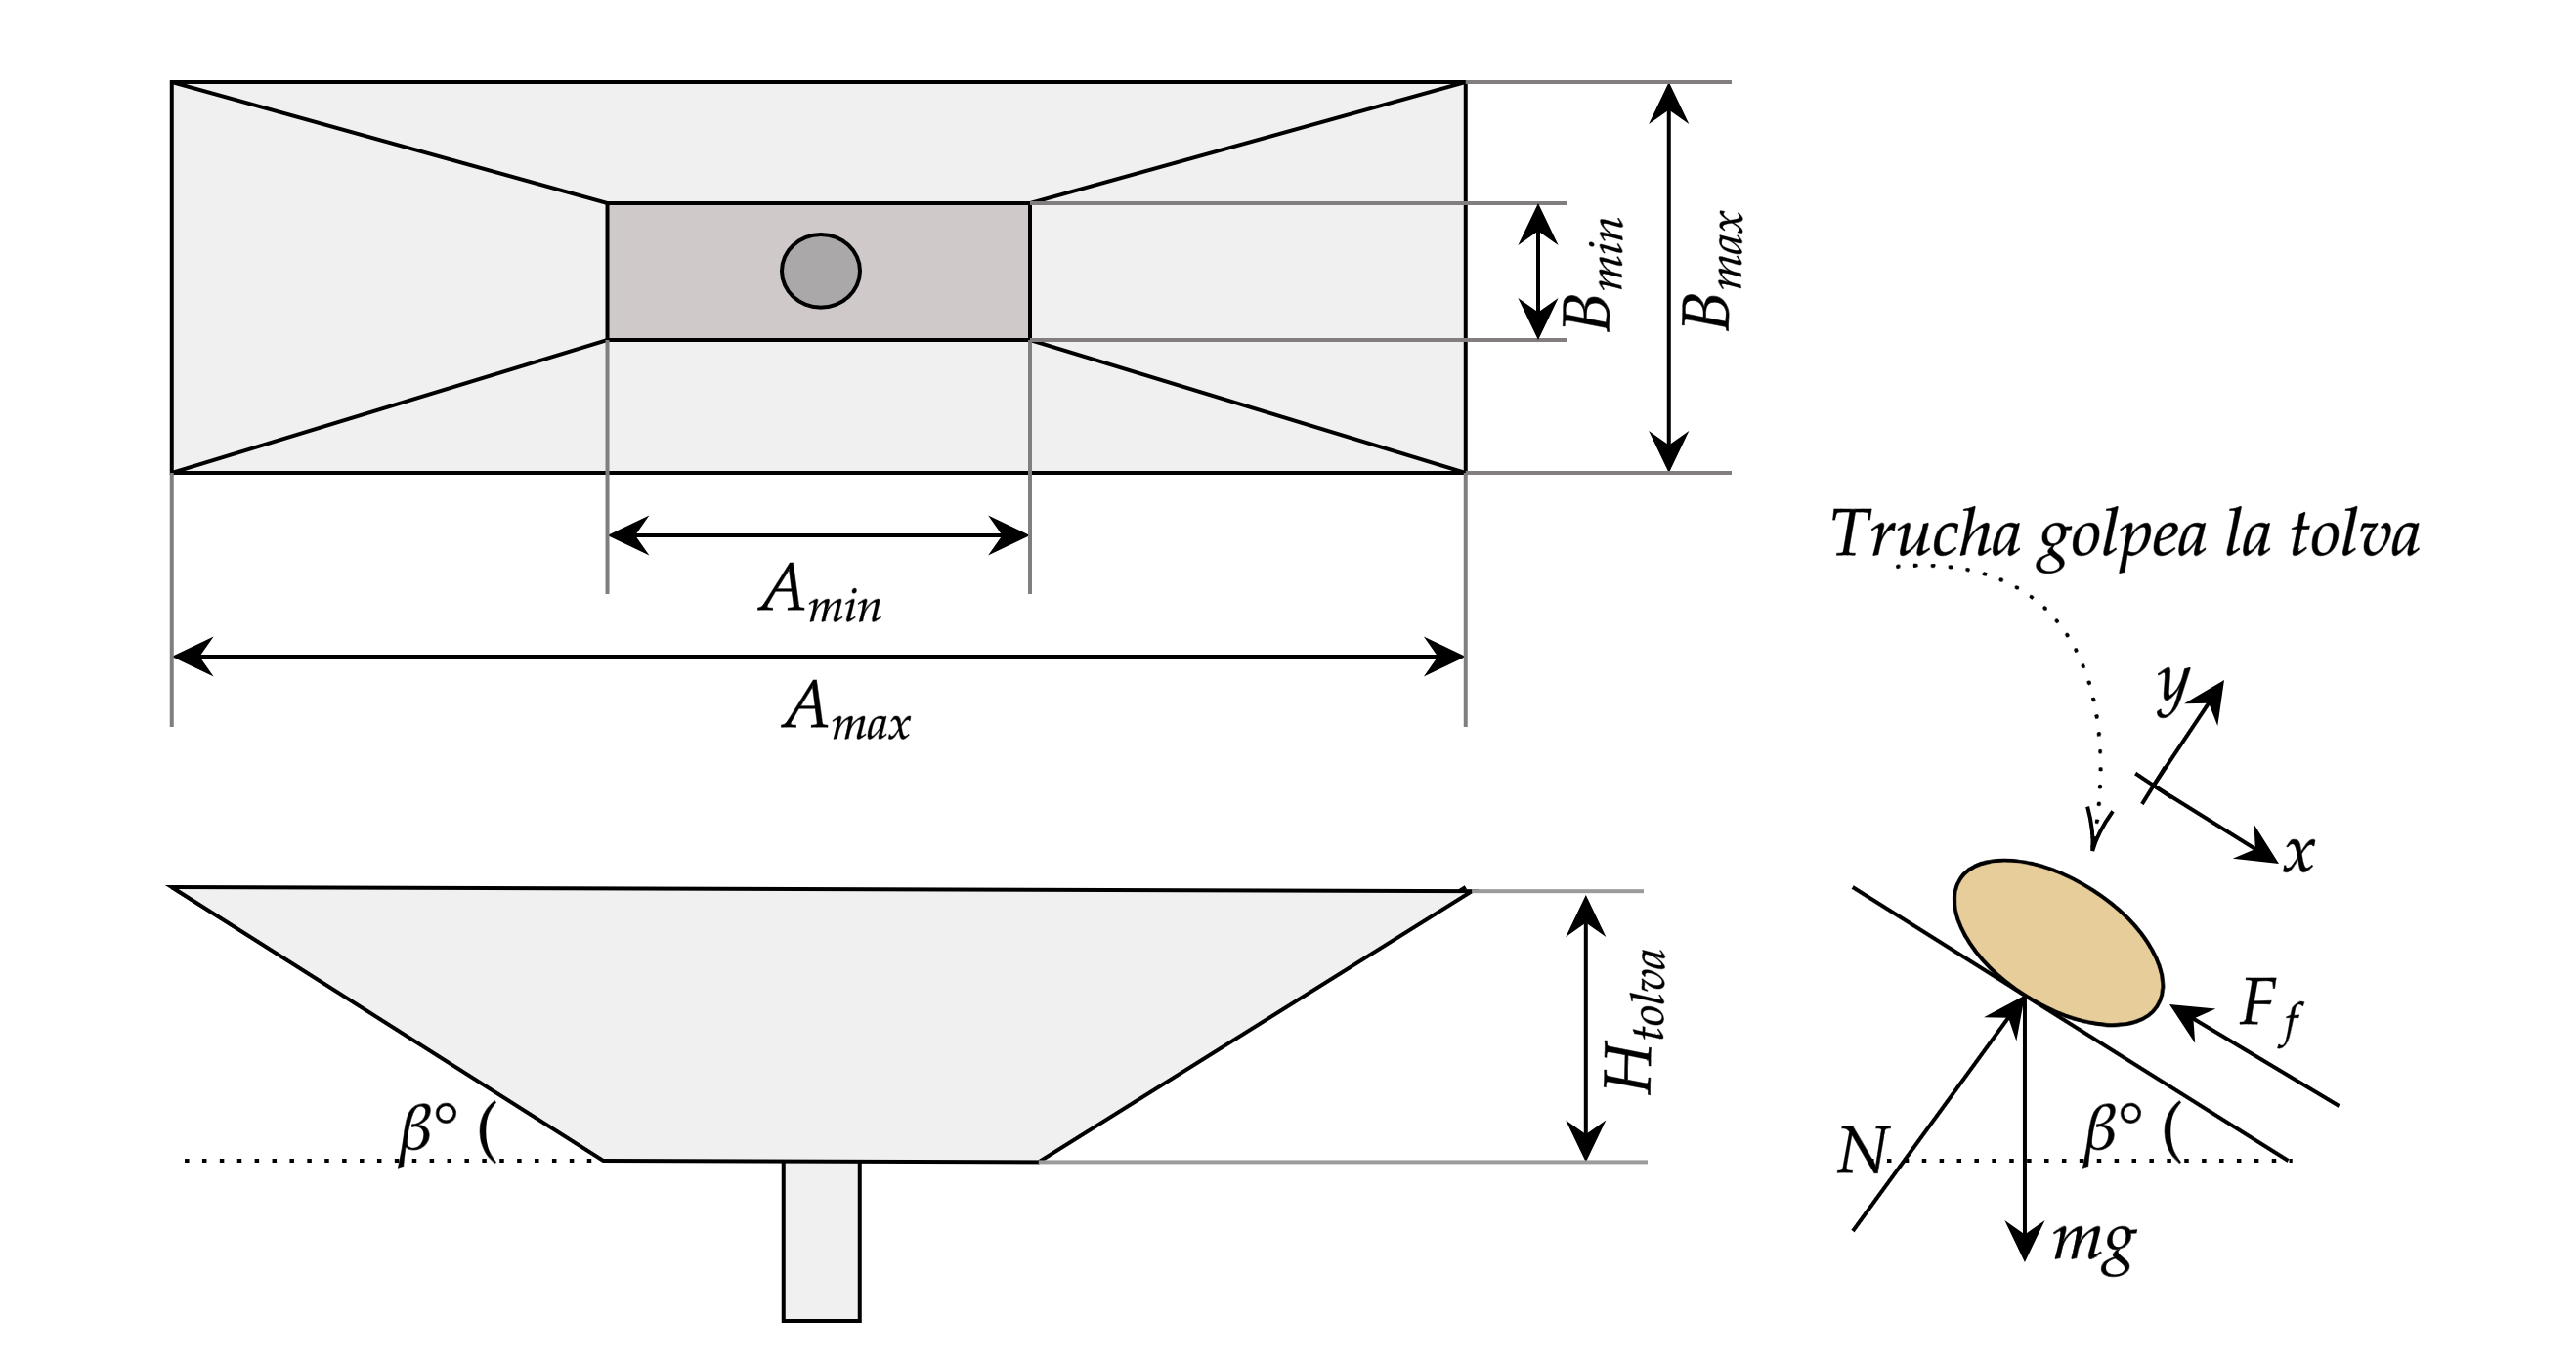
\includegraphics[width=1\textwidth]{chapter5/calculo de dimensiones y angulo de la tolva.png}
	\caption{Cálculo de dimensiones y ángulo de la tolva}
	\begin{myflushleftportland}
		Fuente: Elaboración propia.
	\end{myflushleftportland}
	\label{fig:calculo de dimensiones y angulo de la tolva}
\end{myfigure}

Parte de la Figura \ref{fig:calculo de dimensiones y angulo de la tolva} muestra el diagrama de cuerpo libre del cual se extrae la fuerza de fricción ($F_{f}$) y la fuerza normal ($N$) que se muestran en la Ecuación \ref{eq:calculo de angulo de la tolva}. Las leyes de Newton se muestran en la Ecuación \ref{eq:leyes de newton}. 

\begin{myequation}\label{eq:leyes de newton}
	\begin{split}
		F_{R}=m*a \\
		\sum_{0}^{n}F_{x,y,z}=0
	\end{split}
\end{myequation}

\begin{myequation}\label{eq:calculo de angulo de la tolva}
	\begin{split}
		F_{f}=\mu*N  \\
		\sum_{}^{}F_{y}=N-mg*cos(\beta)=0
	\end{split}
\end{myequation}

Luego, se reemplazan la Ecuación \ref{eq:calculo de angulo de la tolva} en la Ecuación \ref{eq:leyes de newton} y se obtiene la Ecuación \ref{eq:calculo de angulo de la tolva2}. La variable a despejar es la aceleración en el eje x ($\ddot{x}$).

\begin{myequation}\label{eq:calculo de angulo de la tolva2}
	\begin{split}
		mg*sin(\beta)-F_{f}&=m*\ddot{x} \\
		mg*sin(\beta)-\mu_{k}*mg*cos(\beta)&=m*\ddot{x} \\
		g*sin(\beta)-g*\mu_{k}*cos(\beta)&=\ddot{x}
	\end{split}
\end{myequation}

Para disminuir el impacto de la trucha sobre la tolva o sobre las tuberías interiores se debe disminuir la aceleración de la trucha al ser depositada en la tolva. La Figura \ref{fig:grafico angulo de tolva vs aceleracion} muestra la ecuación que relaciona la aceleración con el ángulo de elevación de la pared de la tolva. Consecuentemente, se escoge un ángulo ($\beta=30^\circ$) para tener una aceleración aproximadamente nula ($\ddot{x}\approx0$). Se considera $\mu_{k}=0.57$ para el material escogido en la sección \ref{sssec:seleccion de materiales de fabricacion}. Consecuentemente, se calculan los valores de $A_{max}\approx{900} mm.$ y $B_{max}\approx{700} mm.$, respectivamente.

% Material escogido Acero inoxidable

\begin{myfigure}[H]
	\centering
	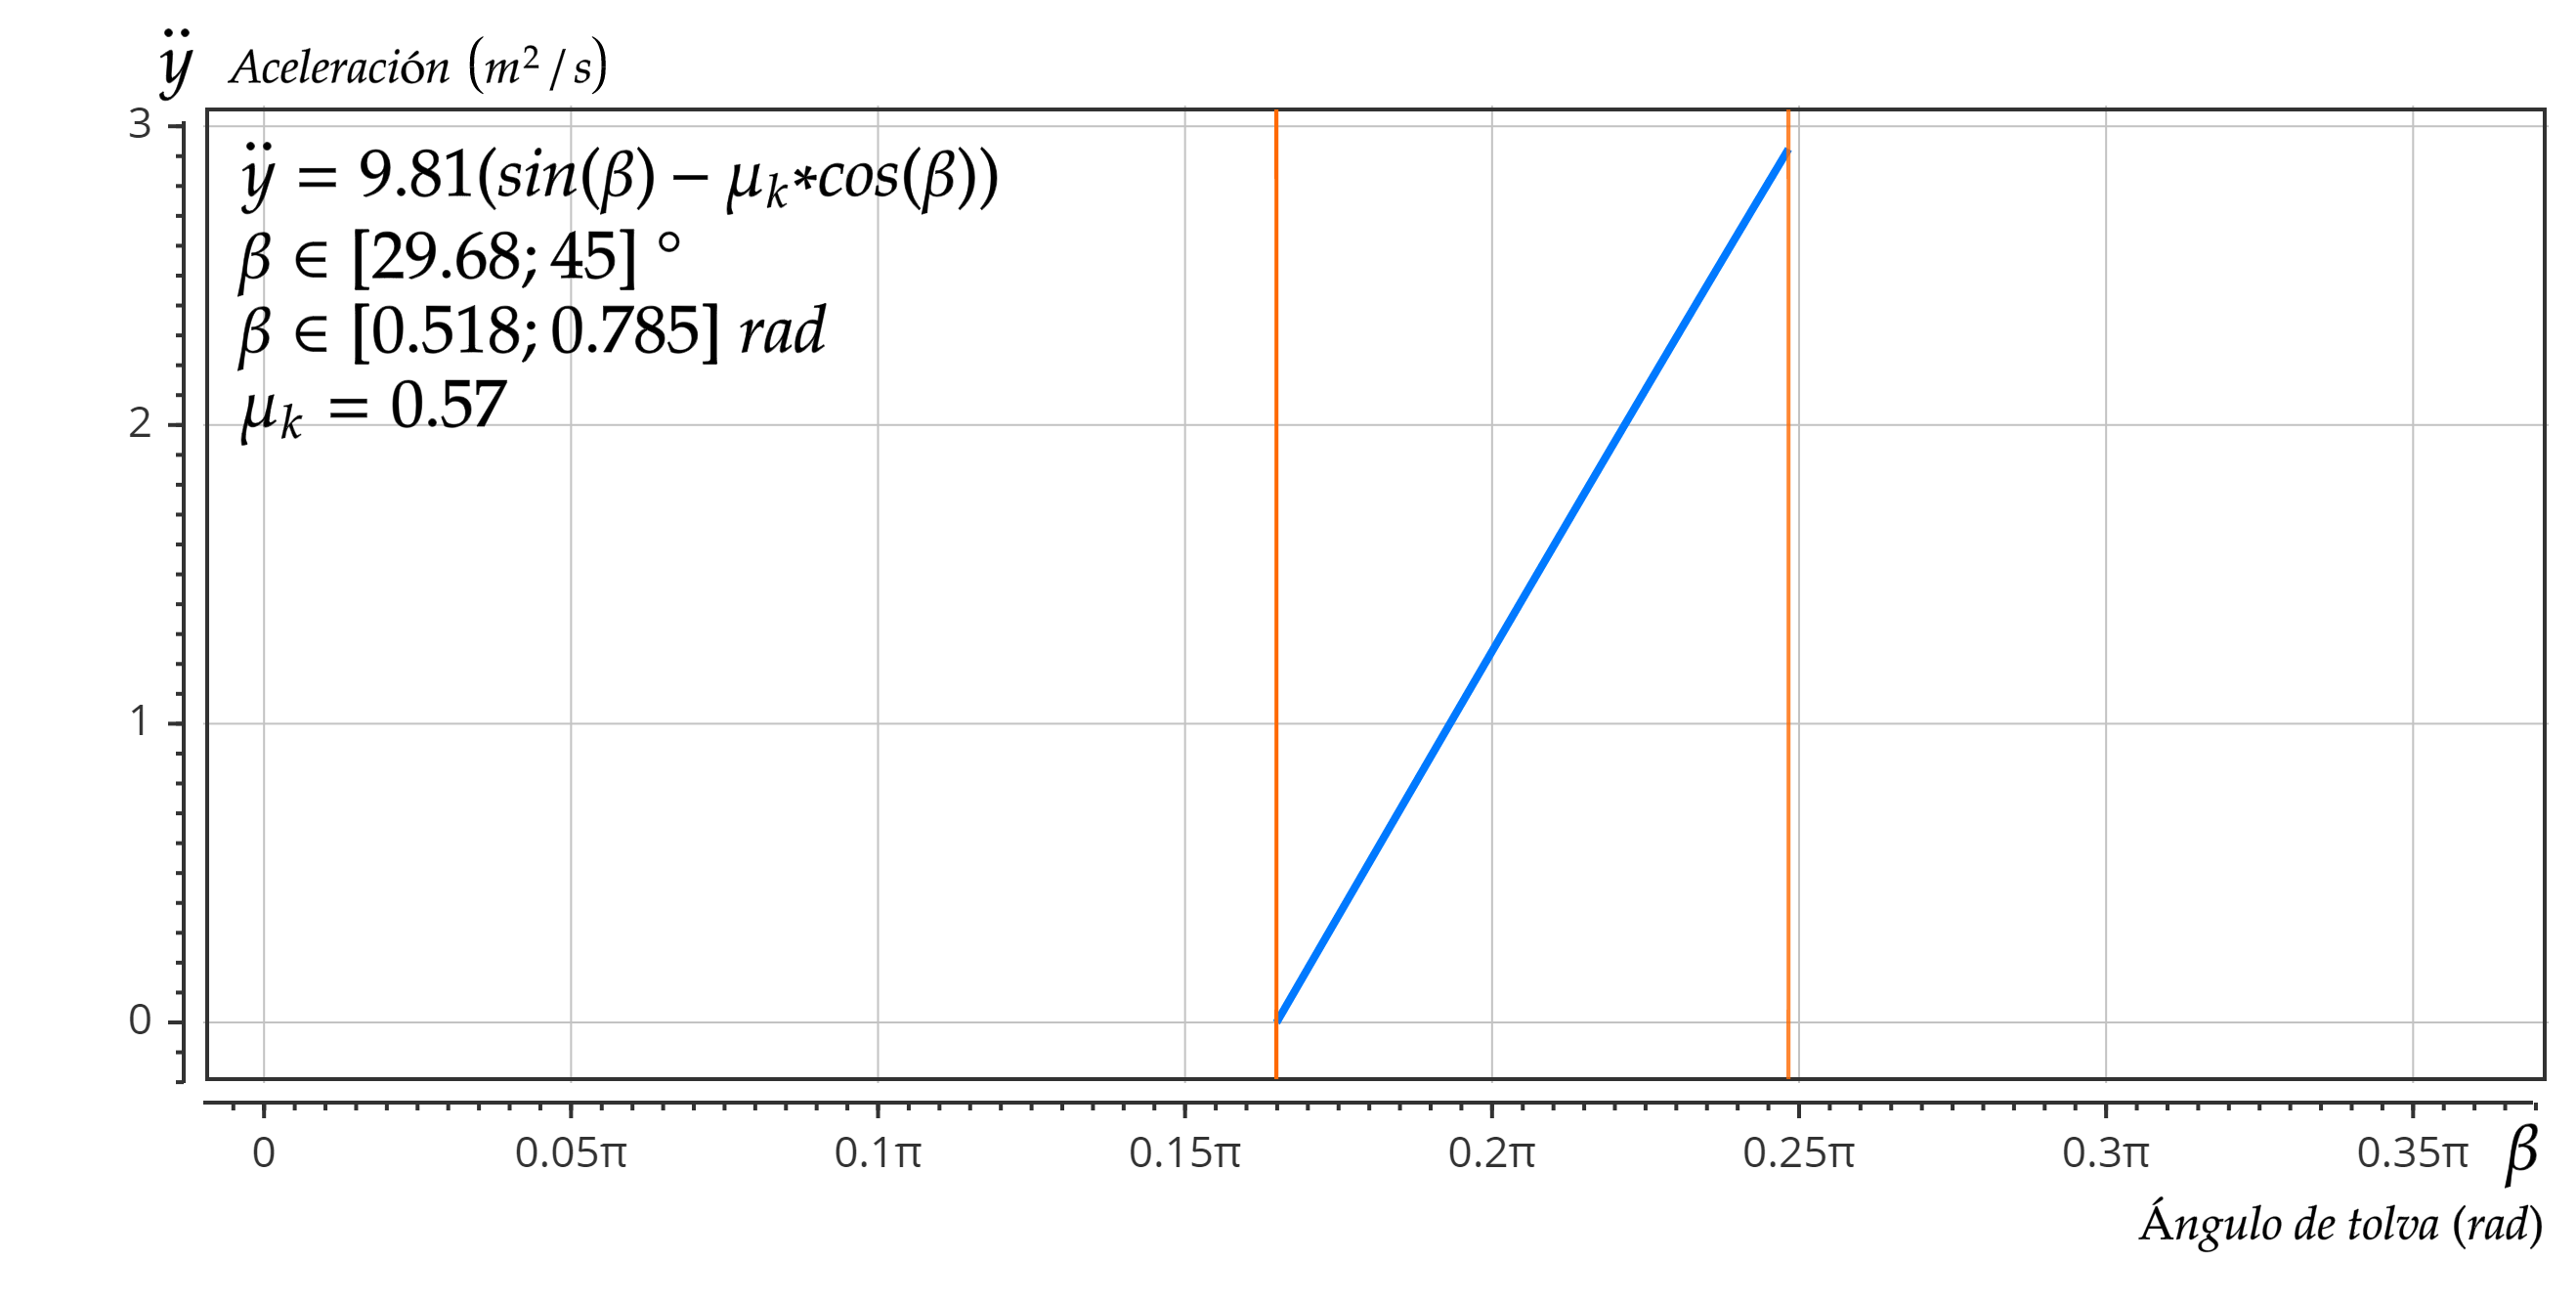
\includegraphics[width=1\textwidth]{chapter5/grafico angulo de tolva vs aceleracion.png}
	\caption{Ángulo de tolva vs aceleración en la trucha}
	\begin{myflushleftportland}
		Fuente: Elaboración propia.
	\end{myflushleftportland}
	\label{fig:grafico angulo de tolva vs aceleracion}
\end{myfigure}

%% NUEVO SUBSECCION X.X.X.X
\subsubsection{Selección de reja accionada por motor}

Esta compuerta puede ser reemplazada por una tapa para la tolva de recepción de truchas. En el presente trabajo se decide optar por eliminar este componente.

\textcolor{blue}{[BORRADOR] ¿Se puede eliminar este inciso en caso no lo use? [/BORRADOR]} 

%% NUEVO SUBSECCION X.X.X.X
\subsubsection{Diseño de subsistema de tuberías}

Las tuberías del sistema tienen como propósito abastecer de un caudal a la máquina.

\textcolor{blue}{[BORRADOR] Explicar en subsitema de tuberías luego de definir los componentes como bombas de agua o electrovalvulas [/BORRADOR]} 

\begin{itemize}
	
	\item \textbf{Diseño de tuberías}
	
	\textcolor{blue}{[BORRADOR] Explicar características y requerimientos técnicos que se necesitarán en las tuberías [/BORRADOR]} 
	
	\begin{myfigure}[H]
		\centering
		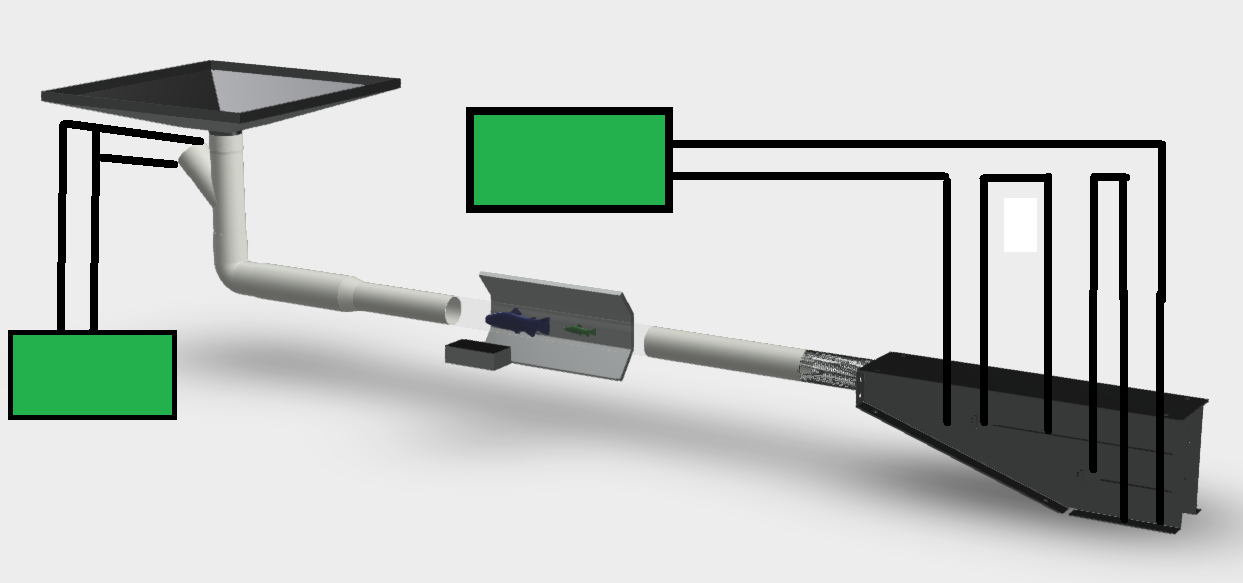
\includegraphics[width=1\textwidth]{chapter5/concepto optimo tuberias.png}
		\caption{Diseño de tuberías para el concepto óptimo}
		\begin{myflushleftportland}
			Fuente: Elaboración propia.
		\end{myflushleftportland}
		\label{fig:concepto optimo tuberias}
	\end{myfigure}
	
	\item \textbf{Diseño de filtro único incluido}
	
	\textcolor{blue}{[BORRADOR] Explicar características y requerimientos técnicos que se necesita para que pase una trucha por vez [/BORRADOR]} 
	
	\begin{myfigure}[H]
		\centering
		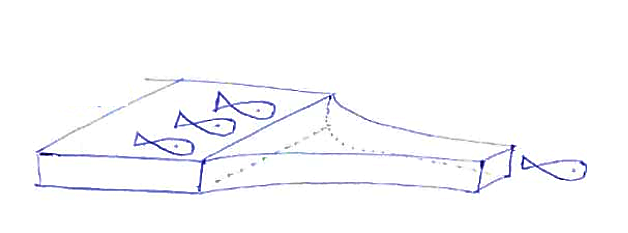
\includegraphics[width=0.25\textwidth]{chapter5/filtro unico.png}
		\caption{Filtro único}
		\begin{myflushleftportland}
			Fuente: Elaboración propia.
		\end{myflushleftportland}
		\label{fig:filtro unico}
	\end{myfigure}
	
	\item \textbf{Selección de caudales apropiados} 
	
	En la Sección \ref{sssec:seleccion de microcontrolador} se calculó la velocidad máxima, aproximada, de nado de las truchas arcoíris: $16 (cm/s)$. La Ecuación \ref{eq:calculo de caudal maximo} toma el valor de \textit{$v_{max}=16 (cm/s)$}  y el 
	
	\begin{myequation}\label{eq:calculo de caudal maximo}
		\begin{split}
			Q_{max} & = v_{max}*A \\
			Q_{max} & = 16*\frac{\pi}{4}*(r_{int})^2 \\
			Q_{max} & = 16*\frac{\pi}{4}*(9.1)^2 \\
			Q_{max} & = 1040.62 
		\end{split}		
	\end{myequation}

	Donde: $Q_{max} (cm^3/s)$ es el caudal máximo, $v_{max} (cm/s)$ es la velocidad máxima del agua, $r_{int} (cm)$.
	
	Lorem ipsum dolor sit amet, consectetur adipiscing elit, sed do eiusmod tempor incididunt ut labore et dolore magna aliqua. Lacus sed turpis tincidunt id aliquet. Nunc aliquet bibendum enim facilisis gravida neque convallis a. Ut tellus elementum sagittis vitae et leo duis ut diam. Dolor sit amet consectetur adipiscing elit ut aliquam purus sit.	
	
	
	\item \textbf{Selección de las electroválvulas}
	
	Los valores límites que se tendrían que controlar mediante las electroválvulas pertenecen al rango $[0;12345] (m^3/s)$. En la Tabla \ref{tab:tabla comparativa de electrovalvulas} se muestran algunas marcas que cumplen con estos requerimientos.
	
	
	\begin{mytable}[H]
		\centering
		\caption{Tabla comparativa de electroválvulas}
		\label{tab:tabla comparativa de electrovalvulas}
		\begin{tabular}{l|c|c|c|c|}
			\cline{2-5}
			\multicolumn{1}{c|}{\textbf{}}            & \textbf{\begin{tabular}[c]{@{}c@{}}Requisitos\\ mínimos\end{tabular}} & \textbf{1} & \textbf{2} & \textbf{3} \\ \hline
			\multicolumn{1}{|l|}{\textbf{Figura}}   & -   
			&
			\begin{minipage}{\mythirdmaxsizeofcontenttable}
				\centering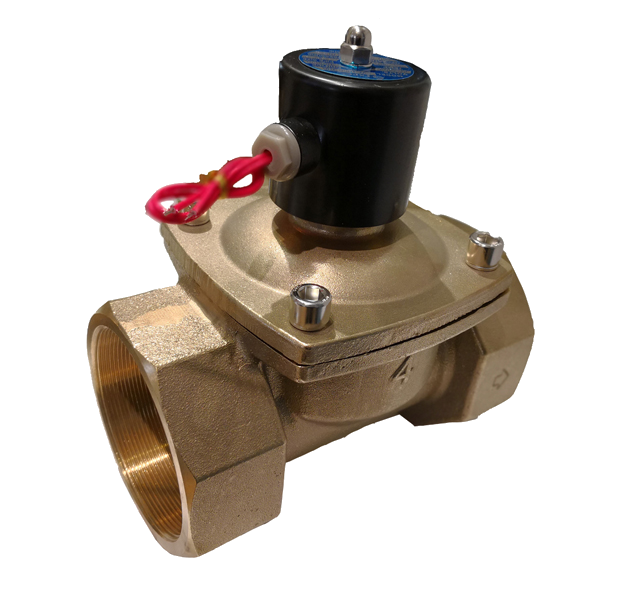
\includegraphics[width=\mythirdmaxsizeimageinsidetable]{chapter5/tablas comparativas/electrovalvula 1.png} \\ 
				%\begin{myflushcenter}
				%	{\footnotesize Nombre imagen}
				%\end{myflushcenter}
			\end{minipage} 
			&
			\begin{minipage}{\mythirdmaxsizeofcontenttable}
				\centering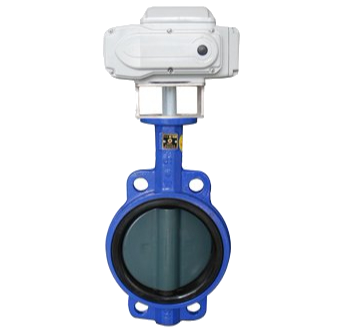
\includegraphics[width=\mythirdmaxsizeimageinsidetable]{chapter5/tablas comparativas/electrovalvula 2.png} \\ 
				%\begin{myflushcenter}
				%	{\footnotesize Nombre imagen}
				%\end{myflushcenter}
			\end{minipage} 
			&
			\begin{minipage}{\mythirdmaxsizeofcontenttable}
				\centering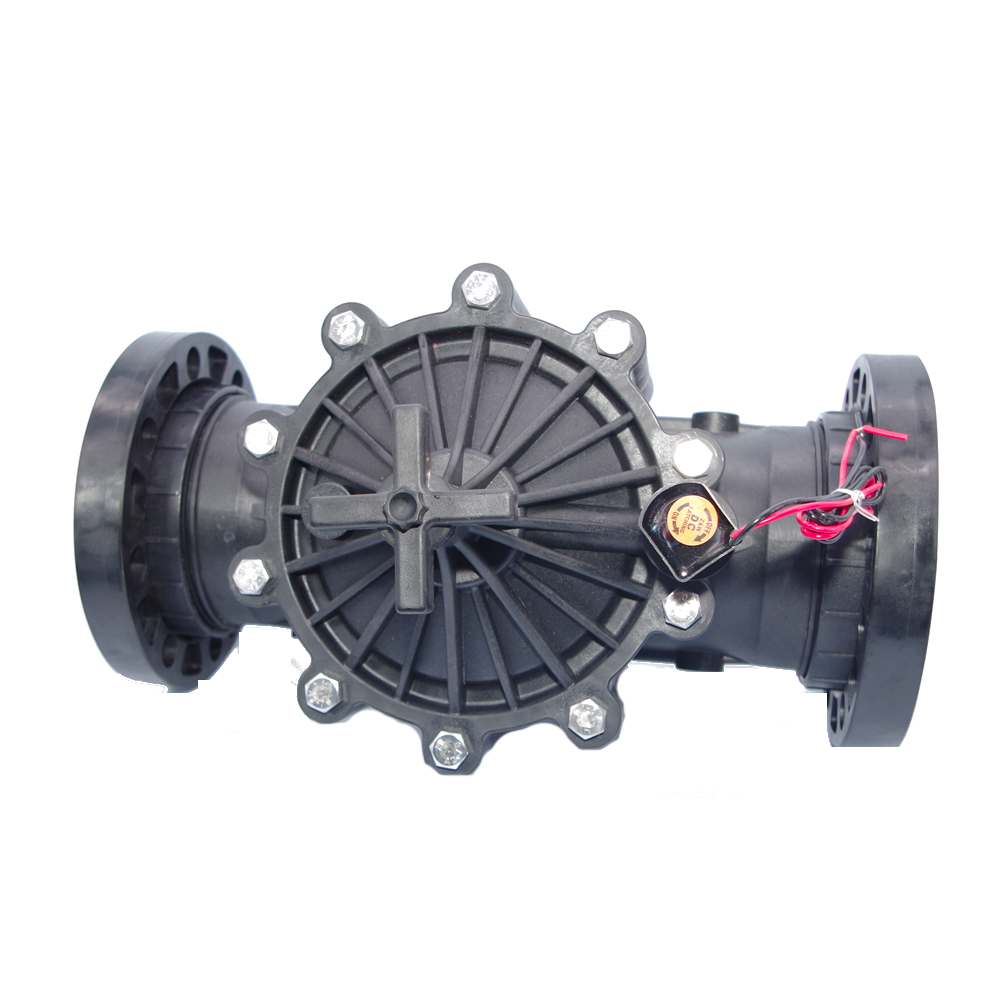
\includegraphics[width=\mythirdmaxsizeimageinsidetable]{chapter5/tablas comparativas/electrovalvula 3.png} \\ 
				%\begin{myflushcenter}
				%	{\footnotesize Nombre imagen}
				%\end{myflushcenter}
			\end{minipage}	\\ \hline
			\multicolumn{1}{|l|}{\textbf{Fabricante}} & 8                                                                     & 9          & 10         & 11         \\ \hline
			\multicolumn{1}{|l|}{\textbf{A}}          & 12                                                                    & 13         & 14         & 15         \\ \hline
			\multicolumn{1}{|l|}{\textbf{B}}          & 16                                                                    & 17         & 18         & 19         \\ \hline
			\multicolumn{1}{|l|}{\textbf{C}}          & 20                                                                    & 21         & 22         & 23         \\ \hline
			\multicolumn{1}{|l|}{\textbf{D}}          & 24                                                                    & 25         & 26         & 27         \\ \hline
			\multicolumn{1}{|l|}{\textbf{E}}          & 32                                                                    & 33         & 34         & 35         \\ \hline
		\end{tabular}	
		\begin{flushleft}			
			Fuente: Imágenes de dominio público y elaboración propia. 
		\end{flushleft}
	\end{mytable}
	
	
	[BORRADOR]Las características técnicas que se muestran en la Tabla XXX muestran que ........ ........... ............. [/BORRADOR]
	 
	
	[BORRADOR] El actuador modelo XXX cumple con los requerimientos de la velocidad de movimiento que no puede ser demasiado lenta porque automatizar el proceso no sería óptimo, por lo que al final terminamos optando por el que tiene menor costo. [/BORRADOR]
	
	\item \textbf{Control de los caudales de agua}
	
	Los caudales que generan las bombas de agua sirven para impulsar a las truchas por el interior de la máquina. 
	
	
	\begin{myfigure}[H]
		\centering
		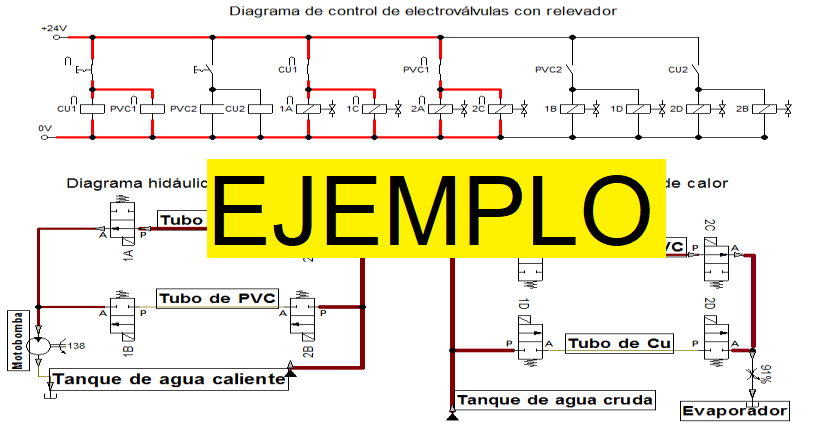
\includegraphics[width=1\textwidth]{chapter5/diagrama de control de electrovalvulas.png}
		\caption{Diagrama de control de electrovalvulas}
		\begin{myflushleftportland}
			Fuente: Elaboración propia.
		\end{myflushleftportland}
		\label{fig:diagrama de control de electrovalvulas}
	\end{myfigure}
	
	Lacus sed turpis tincidunt id aliquet. Nunc aliquet bibendum enim facilisis gravida neque convallis a. Ut tellus elementum sagittis vitae et leo duis ut diam. Dolor sit amet consectetur adipiscing elit ut aliquam purus sit. 
	
	\begin{myfigure}[H]
		\centering
		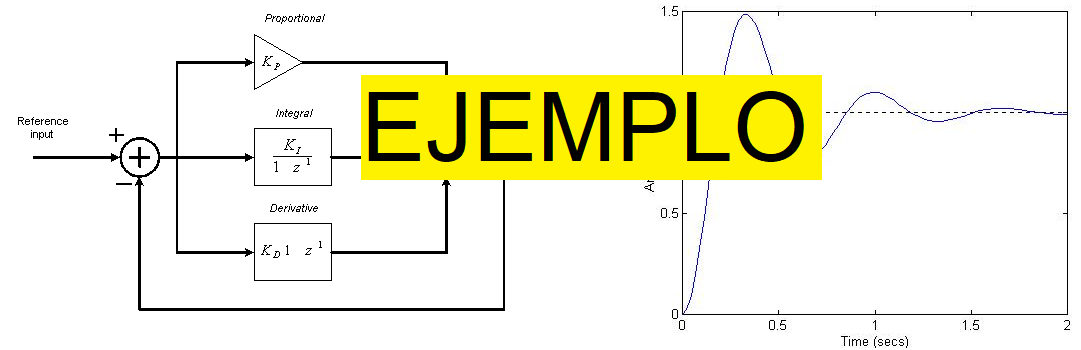
\includegraphics[width=1\textwidth]{chapter5/control electrovalvulas pid.png}
		\caption{Control PID de una electrovalvula}
		\begin{myflushleftportland}
			Fuente: Elaboración propia.
		\end{myflushleftportland}
		\label{fig:control electrovalvulas pid}
	\end{myfigure}
	
	Lacus sed turpis tincidunt id aliquet. Nunc aliquet bibendum enim facilisis gravida neque convallis a. Ut tellus elementum sagittis vitae et leo duis ut diam. Dolor sit amet consectetur adipiscing elit ut aliquam purus sit. 
	
	
\end{itemize}

%% NUEVO SUBSECCION X.X.X.X
\subsubsection{Selección de bomba de agua sumergible}


En la subsección anterior \textit{"Diseño de subsistema de tuberías"} se calcularon los caudales apropiados para el sistema. La bomba de agua sumergible se selecciona de acuerdo a características técnicas como potencia, consumo de energía, horas de uso continuo, entre otras que se exponen en la Tabla \ref{tab:tabla comparativa de bombas de agua sumergibles}.


\begin{mytable}[H]
	\centering
	\caption{Tabla comparativa de bombas de agua sumergibles.}
	\label{tab:tabla comparativa de bombas de agua sumergibles}
	\begin{tabular}{l|c|c|c|c|}
		\cline{2-5}
		\multicolumn{1}{c|}{\textbf{}}            & \textbf{\begin{tabular}[c]{@{}c@{}}Requisitos\\ mínimos\end{tabular}} & \textbf{1} & \textbf{2} & \textbf{3} \\ \hline
		\multicolumn{1}{|l|}{\textbf{Figura}}     & -                                                                     
		&
		\begin{minipage}{\mythirdmaxsizeofcontenttable}
			\centering
\includegraphics[width=\mythirdmaxsizeimageinsidetable]{chapter5/tablas comparativas/bomba de agua sumergible 1.png} \\ 
			%\begin{myflushcenter}
			%	{\footnotesize Nombre imagen}
			%\end{myflushcenter}
		\end{minipage} 
		&
		\begin{minipage}{\mythirdmaxsizeofcontenttable}
			\centering
\includegraphics[width=\mythirdmaxsizeimageinsidetable]{chapter5/tablas comparativas/bomba de agua sumergible 2.png} \\ 
			%\begin{myflushcenter}
			%	{\footnotesize Nombre imagen}
			%\end{myflushcenter}
		\end{minipage} 
		&
		\begin{minipage}{\mythirdmaxsizeofcontenttable}
			\centering
\includegraphics[width=\mythirdmaxsizeimageinsidetable]{chapter5/tablas comparativas/bomba de agua sumergible 3.png} \\ 
			%\begin{myflushcenter}
			%	{\footnotesize Nombre imagen}
			%\end{myflushcenter}
		\end{minipage} 
		\\ \hline
		\multicolumn{1}{|l|}{\textbf{Fabricante}} & 8                                                                     & 9          & 10         & 11         \\ \hline
		\multicolumn{1}{|l|}{\textbf{A}}          & 12                                                                    & 13         & 14         & 15         \\ \hline
		\multicolumn{1}{|l|}{\textbf{B}}          & 16                                                                    & 17         & 18         & 19         \\ \hline
		\multicolumn{1}{|l|}{\textbf{C}}          & 20                                                                    & 21         & 22         & 23         \\ \hline
		\multicolumn{1}{|l|}{\textbf{D}}          & 24                                                                    & 25         & 26         & 27         \\ \hline
		\multicolumn{1}{|l|}{\textbf{E}}          & 32                                                                    & 33         & 34         & 35         \\ \hline
	\end{tabular}
	\begin{flushleft}	
		Fuente: Imágenes de dominio público y elaboración propia.
	\end{flushleft}
\end{mytable}

[BORRADOR] El actuador lineal modelo XXX cumple con los requerimientos de la velocidad de movimiento que no puede ser demasiado lenta porque automatizar el proceso no sería óptimo, por lo que al final terminamos optando por el que tiene menor costo. [/BORRADOR]


%% NUEVO SUBSECCION X.X.X.X
\subsubsection{Diseño de subsistema de distribución de truchas}

Luego del proceso de procesamiento de imágenes el sistema mediante el algoritmo de clasificación dirige a la trucha en tránsito a la salida correspondiente en el mecanismo de distribución de truchas. Dicho mecanismo recibe a la trucha y debe redirigir mediante un juego de compuertas a tres salidas que a su vez se impulsan mediante un caudal a sus respectivas jaulas flotantes.

\begin{itemize}
	
	\item \textbf{Cálculo de fuerza y velocidad de compuertas}
	La fuerza necesaria es simplemente el giro de la compuerta que está unida a un eje y a su vez al mecanismo de engranajes con el servomotor.
	
	\begin{myfigure}[H]
		\centering
		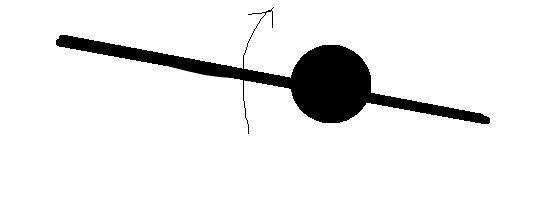
\includegraphics[width=1\textwidth]{chapter5/compuerta.png}
		\caption{Compuerta}
		\begin{myflushleftportland}
			Fuente: Elaboración propia.
		\end{myflushleftportland}
		\label{fig:compuerta}
	\end{myfigure}
	
	La velocidad de compuertas debe ir acorde a la distancia entre una trucha y la siguiente a esta. 
	
	\begin{myfigure}[H]
		\centering
		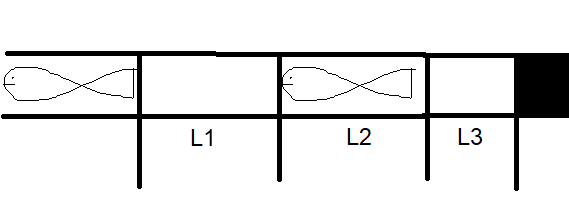
\includegraphics[width=1\textwidth]{chapter5/velocidad de compuerta.png}
		\caption{Velocidad de compuerta}
		\begin{myflushleftportland}
			Fuente: Elaboración propia.
		\end{myflushleftportland}
		\label{fig:velocidad de compuerta}
	\end{myfigure}

	Ut tellus elementum sagittis vitae et leo duis ut diam. Dolor sit amet consectetur adipiscing elit ut aliquam purus sit. 
	
	\begin{myequation}\label{eq:calculo de tiempo necesario}
		\begin{split}
			L_1+L_2+L_3 &= t * v
		\end{split}		
	\end{myequation}

	Ut tellus elementum sagittis vitae et leo duis ut diam. Dolor sit amet consectetur adipiscing elit ut aliquam purus sit. 

	
	\item \textbf{Selección de servomotores}
		
	Calcular: \\
	- Torque necesario \\
	- Condiciones de uso (estará en agua) \\
	- Tiempo de uso \\
	
	La selección de los servomotores depende del propósito en la función que se encuentre................
	
	Este servomotor acciona la compuerta presentada en la Figura \ref{fig:compuerta}. El torque necesario del eje es $T_{max}=X (M*mm)$  y gracias al mecanismo de engranajes puede reducirse a $T_{max_2}=Y (M*mm)$ En la Tabla \ref{tab:tabla comparativa de servomotores} se muestra una comparación técnica entre tres servomotores que cumplen los requerimientos técnicos y conceptuales.
	
	\begin{mytable}[H]
		\centering
		\caption{Tabla comparativa de servomotores.}
		\label{tab:tabla comparativa de servomotores}
		\begin{tabular}{l|c|c|c|c|}
			\cline{2-5}
			\multicolumn{1}{c|}{\textbf{}}            & \textbf{\begin{tabular}[c]{@{}c@{}}Requisitos\\ mínimos\end{tabular}} & \textbf{1} & \textbf{2} & \textbf{3} \\ \hline
			\multicolumn{1}{|l|}{\textbf{Figura}}     & -                                                                     
			&
			\begin{minipage}{\mythirdmaxsizeofcontenttable}
				\centering
\includegraphics[width=\mythirdmaxsizeimageinsidetable]{chapter5/tablas comparativas/servomotor 1.png} \\ 
				%\begin{myflushcenter}
				%	{\footnotesize Nombre imagen}
				%\end{myflushcenter}
			\end{minipage} 
			&
			\begin{minipage}{\mythirdmaxsizeofcontenttable}
				\centering
\includegraphics[width=\mythirdmaxsizeimageinsidetable]{chapter5/tablas comparativas/servomotor 2.png} \\ 
				%\begin{myflushcenter}
				%	{\footnotesize Nombre imagen}
				%\end{myflushcenter}
			\end{minipage} 
			&
			\begin{minipage}{\mythirdmaxsizeofcontenttable}
				\centering
\includegraphics[width=\mythirdmaxsizeimageinsidetable]{chapter5/tablas comparativas/servomotor 3.png} \\ 
				%\begin{myflushcenter}
				%	{\footnotesize Nombre imagen}
				%\end{myflushcenter}
			\end{minipage} 
			\\ \hline
			\multicolumn{1}{|l|}{\textbf{Fabricante}} & 8                                                                     & 9          & 10         & 11         \\ \hline
			\multicolumn{1}{|l|}{\textbf{A}}          & 12                                                                    & 13         & 14         & 15         \\ \hline
			\multicolumn{1}{|l|}{\textbf{B}}          & 16                                                                    & 17         & 18         & 19         \\ \hline
			\multicolumn{1}{|l|}{\textbf{C}}          & 20                                                                    & 21         & 22         & 23         \\ \hline
			\multicolumn{1}{|l|}{\textbf{D}}          & 24                                                                    & 25         & 26         & 27         \\ \hline
			\multicolumn{1}{|l|}{\textbf{E}}          & 32                                                                    & 33         & 34         & 35         \\ \hline
		\end{tabular}
		\begin{flushleft}	
			Fuente: Imágenes de dominio público y elaboración propia.
		\end{flushleft}
	\end{mytable}
	
	
%	\begin{itemize}
%		
%		%% ANTES HABIA 2 MECANISMOS CON SERVO, AHORA SOLO 1
%		
%		%\item \textbf{Servomotor 1: } Este servomotor apoya en la función de
%		\textit{accionar recepción de truchas}. 
%		
%		\item \textbf{Servomotor de compuerta} 
%		
%	\end{itemize}


	\item \textbf{Diseño de mecanismo servomotor-compuerta} 
	
	Ut tellus elementum sagittis vitae et leo duis ut diam. Dolor sit amet consectetur adipiscing elit ut aliquam purus sit. 
	
	\begin{myfigure}[H]
		\centering
		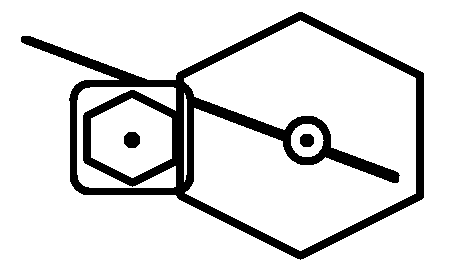
\includegraphics[width=1\textwidth]{chapter5/mecanismo servomotor-compuerta.png}
		\caption{Mecanismo servomotor-compuerta}
		\begin{myflushleftportland}
			Fuente: Elaboración propia.
		\end{myflushleftportland}
		\label{fig:mecanismo servomotor-compuerta}
	\end{myfigure}
	
	Ut tellus elementum sagittis vitae et leo duis ut diam. Dolor sit amet consectetur adipiscing elit ut aliquam purus sit. 
	
	\begin{myfigure}[H]
		\centering
		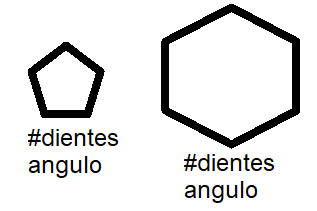
\includegraphics[width=1\textwidth]{chapter5/mecanismo de compuertas engranajes.png}
		\caption{Engranajes del mecanismo de compuertas}
		\begin{myflushleftportland}
			Fuente: Elaboración propia.
		\end{myflushleftportland}
		\label{fig:mecanismo de compuertas engranajes}
	\end{myfigure}
	
	Ut tellus elementum sagittis vitae et leo duis ut diam. Dolor sit amet consectetur adipiscing elit ut aliquam purus sit. 
	
	
	\item \textbf{Diseño de juego de compuertas programables}
	
	Descripción.

\end{itemize}





%% NUEVA SECCIÓN X.X.X
\subsection{Subsistema de procesamiento de imágenes}
\label{ssec:subsistema de procesamiento de imágenes}

Este subsistema consiste obtener una serie de imágenes de una trucha en tránsito e indicar al sistema a dónde debería dirigirse una trucha determinada. El subsistema debe clasificar y contar truchas, con dicha finalidad necesita de la selección de una cámara y generar el ambiente adecuado para obtener las imágenes. Explicado los objetivos del subsistema, en las siguientes líneas se detalla: la selección del sensor infrarrojo, la selección de cámara estéreo, la selección de iluminación adecuada y la selección de algoritmos.

%% NUEVO SUBSECCION X.X.X.X
\subsubsection{Selección del sensor infrarrojo}

El sensor infrarrojo tiene como objetivo activar el algoritmo de detección y conteo de truchas por un determinado periodo de tiempo con la finalidad de evitar un sobre uso de los recursos computacionales. El sensor infrarrojo está unos centímetros antes de la parte que la cámara captura y su posición es como se muestra en las Figura \ref{fig:posicion sensor infrarrojo}.

\begin{myfigure}[H]
	\centering
	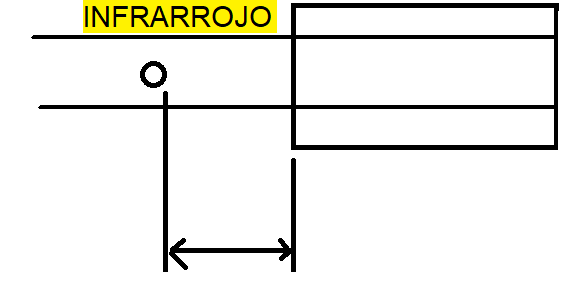
\includegraphics[width=1\textwidth]{chapter5/posicion sensor infrarrojo.png}
	\caption{Posicionamiento del sensor infrarrojo}
	\begin{myflushleftportland}
		Fuente: Elaboración propia.
	\end{myflushleftportland}
	\label{fig:posicion sensor infrarrojo}
\end{myfigure}

Ya que los haces de luz cambian de dirección debido a la refracción\footnote{\cite{Hecht2017}.}, cuando varía de un medio a otro, se calcula esta desviación para la adecuada detección de objetos que pasen por la tubería. La representación gráfica de la situación se expone en la Figura \ref{fig:analisis de posicion de luz infrarroja}.

\begin{myfigure}[H]
	\centering
	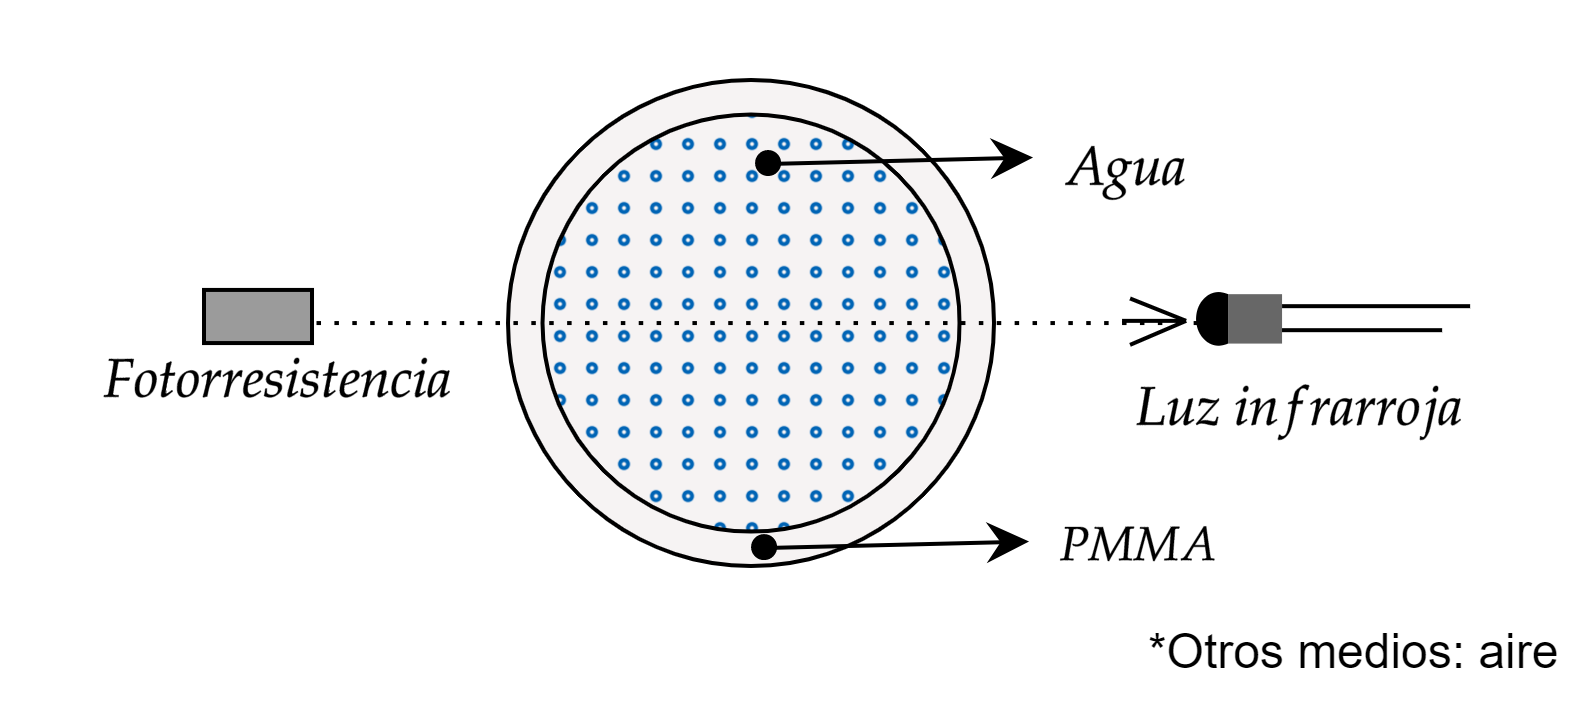
\includegraphics[width=0.75\textwidth]{chapter5/analisis de posicion de luz infrarroja.png}
	\caption{Análisis de posición de luz infrarroja}
	\begin{myflushleftportland}
		Fuente: Elaboración propia.
	\end{myflushleftportland}
	\label{fig:analisis de posicion de luz infrarroja}
\end{myfigure}

El problema se muestra en la Figura \ref{fig:calculo de posicion de luz infrarroja}. Cabe mencionar que se conocen los siguientes valores $n_{PMMA}=1.5$\footnote{Propiedades ópticas mostradas en la Tabla \ref{tab:tabla comparativa de propiedades entre pmma vs pvdf}. \cite{Berins1991}}, $n_{aire}\approx1$, $n_{agua}=1.33$\footnote{Índices de refracción: \cite{Hecht2017}.}, $d_{1}=d_{2}=10 mm.$, $e=3 mm.$ y $d_{int}=85 mm.$ ,y se asume, para simplificar el problema, la emisión de la luz como proveniente de un punto único ($S$).

\begin{myfigure}[H]
	\centering
	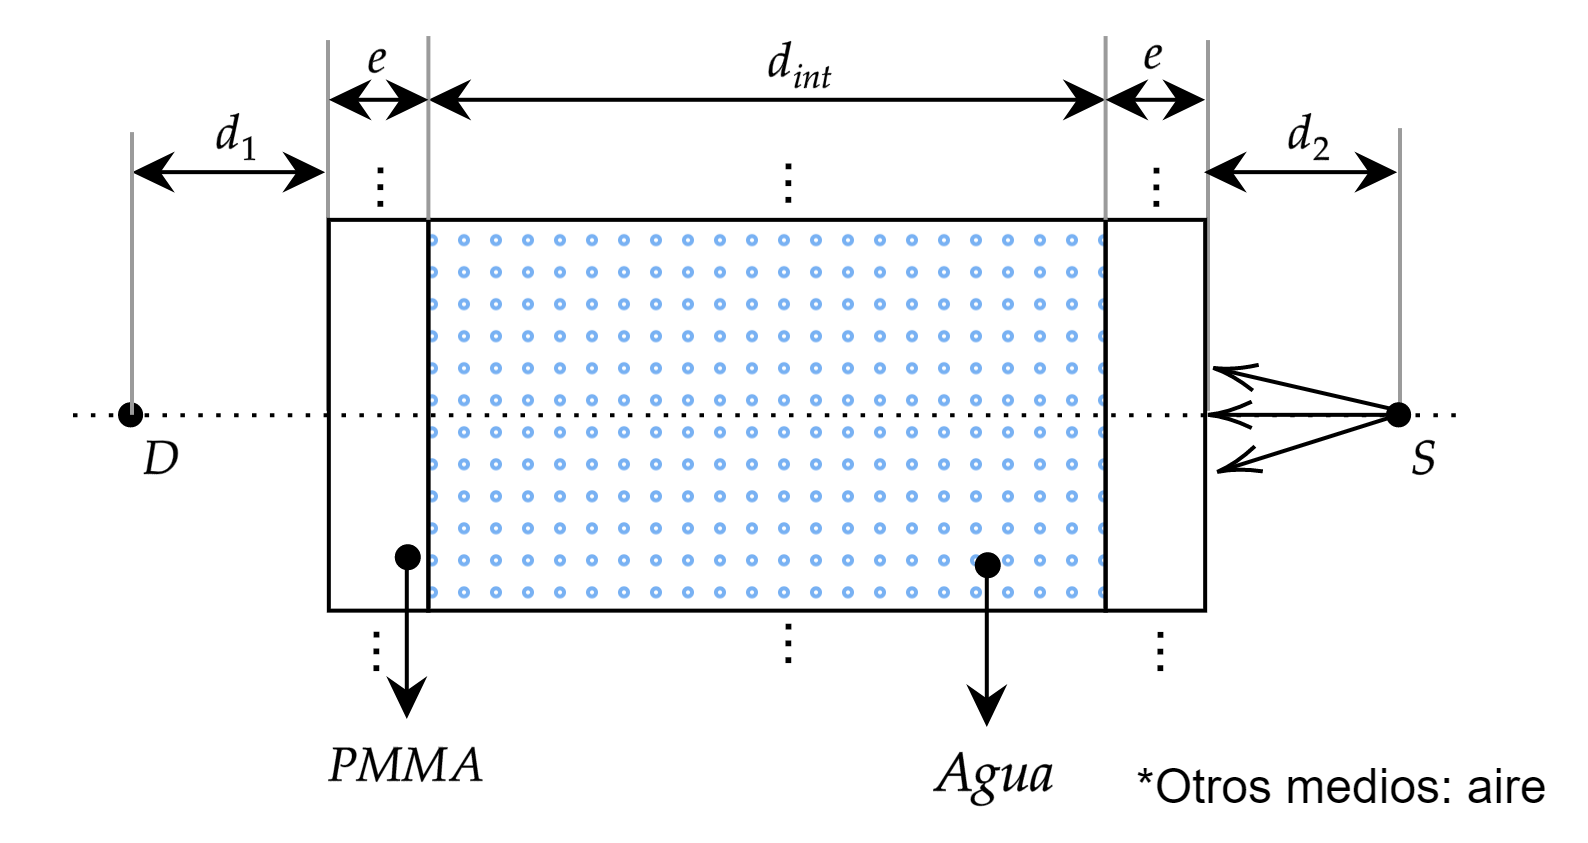
\includegraphics[width=0.75\textwidth]{chapter5/calculo de posicion de luz infrarroja.png}
	\caption{Cálculo de posición de luz infrarroja}
	\begin{myflushleftportland}
		Fuente: Elaboración propia.
	\end{myflushleftportland}
	\label{fig:calculo de posicion de luz infrarroja}
\end{myfigure}

Para el cálculo de desviación de los haces de luz se emplea la ley de refracción, matemáticamente mostrada en la Ecuación \ref{eq:ecuacion de snell}. Donde: $\theta_{i}$ es el ángulo de incidencia respecto a la normal del primer medio, $\theta_{t}$ es el ángulo de refracción respecto a la normal.

\begin{myequation}\label{eq:ecuacion de snell}
	\begin{split}
		n_{i}*sin(\theta_{i})&=n_{t}*sin(\theta_{t})
	\end{split}		
\end{myequation}

En la Figura \ref{fig:calculo distancia maxima de desviacion de haz de luz en condiciones ideales} se analiza el caso crítico cuando $\theta_{1}\approx5^\circ$. Con la Ecuación \ref{eq:ecuacion de snell} se puede calcular las distancias de desviación por refracción. Por ejemplo, En la Ecuación \ref{eq:calculo distancia maxima de desviacion de haz de luz en condiciones ideales} el valor de $h_{x}$ es la distancia proyectada: $h_{x}=d_{x}*tan(\theta_{x})$.

\begin{myfigure}[H]
	\centering
	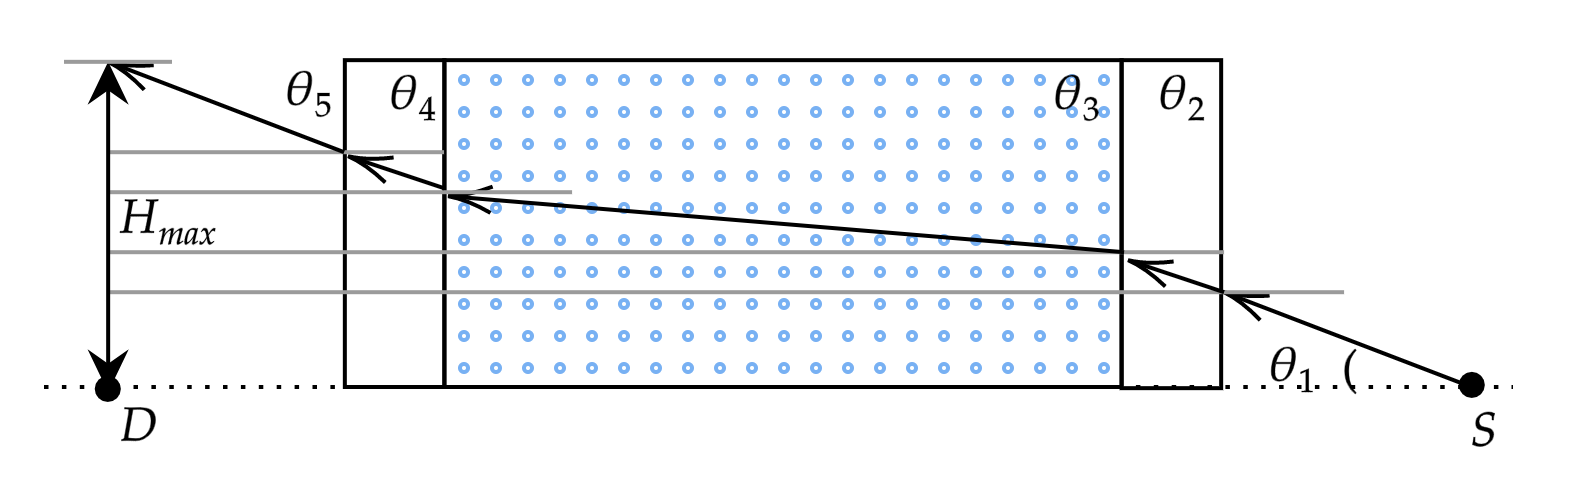
\includegraphics[width=0.75\textwidth]{chapter5/calculo distancia maxima de desviacion de haz de luz en condiciones ideales.png}
	\caption{Cálculo de distancia máxima de desviación de haz de luz en condiciones ideales.}
	\begin{myflushleftportland}
		Fuente: Elaboración propia.
	\end{myflushleftportland}
	\label{fig:calculo distancia maxima de desviacion de haz de luz en condiciones ideales}
\end{myfigure}

\begin{myequation}\label{eq:calculo distancia maxima de desviacion de haz de luz en condiciones ideales}
	\begin{split}
		H_{max}&=h_{1}+h_{2}+h_{3}+h_{4}+h_{5} \\
		H_{max}&=10*tan(\theta_{1})+3*tan(\theta_{2})+85*tan(\theta_{3})+3*tan(\theta_{4})+10*tan(\theta_{5}) \\
		H_{max}&=10*tan(5^\circ)+3*tan(3.33^\circ)+85*tan(3.76^\circ)+3*tan(3.33^\circ)+10*tan(5^\circ) \\
		H_{max}&=7.685 mm.
	\end{split}		
\end{myequation}

Para una óptima recepción se propone llegar como mínimo 75\% de haces de luz. Esto quiere decir que del diámetro ideal del dispositivo receptor debe ser de 15.4 mm y el óptimo 13.33 mm.\footnote{$d_{ideal-receptor}=2*H_{max}=15.4 mm.$ y $d_{75\%-receptor}=\sqrt{0.75*15.4^2}=13.33 mm.$ } Finalmente, los requerimientos mínimos que debe tener el sensor infrarrojo óptimo y comparaciones técnicas de los dispositivos comerciales que cumplen con los requerimientos se muestran en la Tabla \ref{tab:tabla comparativa de sensores infrarrojos}.

\begin{mytable}[H]
	\centering
	\caption{Tabla comparativa de sensores infrarrojos.}
	\label{tab:tabla comparativa de sensores infrarrojos}
	\begin{tabular}{l|c|c|c|c|}
		\cline{2-5}
		\multicolumn{1}{c|}{\textbf{}}            & \textbf{\begin{tabular}[c]{@{}c@{}}Requisitos\\ mínimos\end{tabular}} &
		\multicolumn{1}{|l|}{				
			\begin{minipage}{\mythirdmaxsizeofcontenttable}	
				\textbf{HD-DS25 CM-3MM}
			\end{minipage}
		}&
		\multicolumn{1}{|l|}{				
			\begin{minipage}{\mythirdmaxsizeofcontenttable}	
				\textbf{QT50CM}
			\end{minipage}
		}&
		\multicolumn{1}{|l|}{				
			\begin{minipage}{\mythirdmaxsizeofcontenttable}	
				\textbf{GP2Y0A 21YK0F}
			\end{minipage}
		}  \\ \hline
		\multicolumn{1}{|l|}{\textbf{Figura}} & - 
		&		  
		\begin{minipage}{\mythirdmaxsizeofcontenttable}
			\centering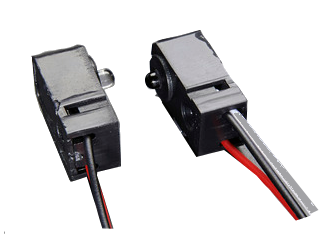
\includegraphics[width=\mythirdmaxsizeimageinsidetable]{chapter5/tablas comparativas/sensor infrarrojo 1.png} \\ 
			%\begin{myflushcenter}
			%	{\footnotesize Nombre imagen}
			%\end{myflushcenter}
		\end{minipage}
		&		  
		\begin{minipage}{\mythirdmaxsizeofcontenttable}
			\centering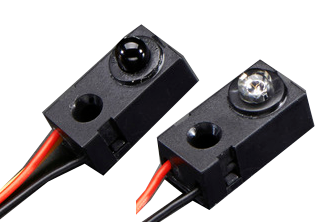
\includegraphics[width=\mythirdmaxsizeimageinsidetable]{chapter5/tablas comparativas/sensor infrarrojo 2.png} \\ 
			%\begin{myflushcenter}
			%	{\footnotesize Nombre imagen}
			%\end{myflushcenter}
		\end{minipage}
		&  
		\begin{minipage}{\mythirdmaxsizeofcontenttable}
			\centering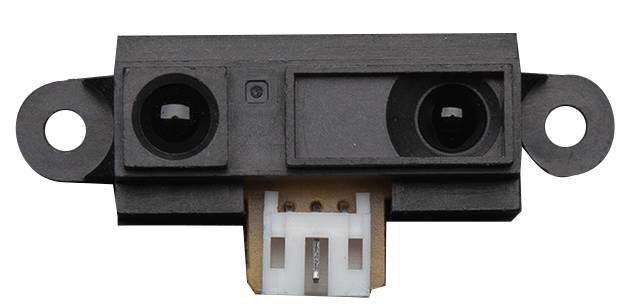
\includegraphics[width=\mythirdmaxsizeimageinsidetable]{chapter5/tablas comparativas/sensor infrarrojo 3.png} \\ 
			%\begin{myflushcenter}
			%	{\footnotesize Nombre imagen}
			%\end{myflushcenter}
		\end{minipage}\\ \hline
		\multicolumn{1}{|l|}{\textbf{Fabricante}} 
		& - & Adafruit & Adafruit & SHARP\\ \hline
		\multicolumn{1}{|l|}{
			\begin{minipage}{\myforthmaxsizeofcontenttable}	
				\textbf{Tipo de comunicación}
			\end{minipage}
		} & Digital & [0;VCC] & [0;VCC] & Analógico         \\ \hline
		\multicolumn{1}{|l|}{
			\begin{minipage}{\myforthmaxsizeofcontenttable}	
				\textbf{Área mínima circular de receptor ($mm^2$)}
			\end{minipage}
		} & 15.4 & 28.27 & 78.54 & 162.86         \\ \hline
		\multicolumn{1}{|l|}{
			\begin{minipage}{\myforthmaxsizeofcontenttable}	
				\textbf{Ángulo de visión/recepción (°)}
			\end{minipage}
		} & 5 & 10 & 10 & -         \\ \hline
		\multicolumn{1}{|l|}{
			\begin{minipage}{\myforthmaxsizeofcontenttable}	
				\textbf{Distancia de detección ($mm.$)}
			\end{minipage}
		} & 170 & [0;250] & [0;500] & [100;800] \\ \hline
		\multicolumn{1}{|l|}{
			\begin{minipage}{\myforthmaxsizeofcontenttable}	
				\textbf{Longitud de onda infrarroja recomendada ($nm$)}
			\end{minipage}
		} & 850 & - & - & 870$\pm$70 \\ \hline
		\multicolumn{1}{|l|}{
			\begin{minipage}{\myforthmaxsizeofcontenttable}	
				\textbf{Voltaje operativo VCC ($V$)}
			\end{minipage}
		} & 5  & [3.0;5.5] & [3.0;5.5] & [4.5;5.5]         \\ \hline
		\multicolumn{1}{|l|}{
			\begin{minipage}{\myforthmaxsizeofcontenttable}	
				\textbf{Consumo de corriente ($mA$)}
			\end{minipage}
		} & -  & 100 & 100 & 30         \\ \hline
		\multicolumn{1}{|l|}{
			\begin{minipage}{\myforthmaxsizeofcontenttable}	
				\textbf{Temperatura operativa (°$C$)}
			\end{minipage}
		} & [-10;60] & [-25;60] & [-25;60] & [-10;60] \\ \hline
		\multicolumn{1}{|l|}{
			\begin{minipage}{\myforthmaxsizeofcontenttable}	
				\textbf{Precio ($S/$)}
			\end{minipage}
		} & - & 7.00 & 23.32 & 53.68 \\ \hline
	\end{tabular}
	\begin{flushleft}	
		Fuente: Marktech Optoelectronics y elaboración propia. Hoja de datos técnico (\textit{Datasheet}) en el Anexo.\\
		Tasa de cambio de USD a PEN: S/ 3.59.
	\end{flushleft}
\end{mytable}

[BORRADOR] El actuador lineal modelo XXX cumple con los requerimientos de la velocidad de movimiento que no puede ser demasiado lenta porque automatizar el proceso no sería óptimo, por lo que al final terminamos optando por el que tiene menor costo. [/BORRADOR]

%% NUEVO SUBSECCION X.X.X.X
\subsubsection{Selección de cámaras} 

En el sistema se emplea dos cámaras con distintos requerimientos técnicos. Por un lado, una cámara estéreo se encarga de capturar imágenes que van a ser procesadas por algoritmos de detección y conteo de truchas. Por otro lado, una cámara normal registra la trayectoria de las truchas que en la distribución de estas a los canales de salida definidos por los algoritmos. 

\begin{itemize}
	
	\item \textbf{Cálculo de distancias apropiadas de las cámaras}
	
	El área que se debe captar sobre el proceso, sin las tuberías transparentes, se representan  en una vista frontal y de perfil en la Figura \ref{fig:distancia entre juego de espejos y camara estereo}. Donde: $d$ es la distancia entre el juego de espejos y la cámara, $\alpha$ es el HDFV\footnote{Campo de visión horizontal.}, $\beta$ es el VDFV\footnote{Campo de visión vertical.}, $A$ es la altura del área proyectada y $L$ es la largo del área proyectada del juego de espejos.
	
	\begin{myfigure}[H]
		\centering
		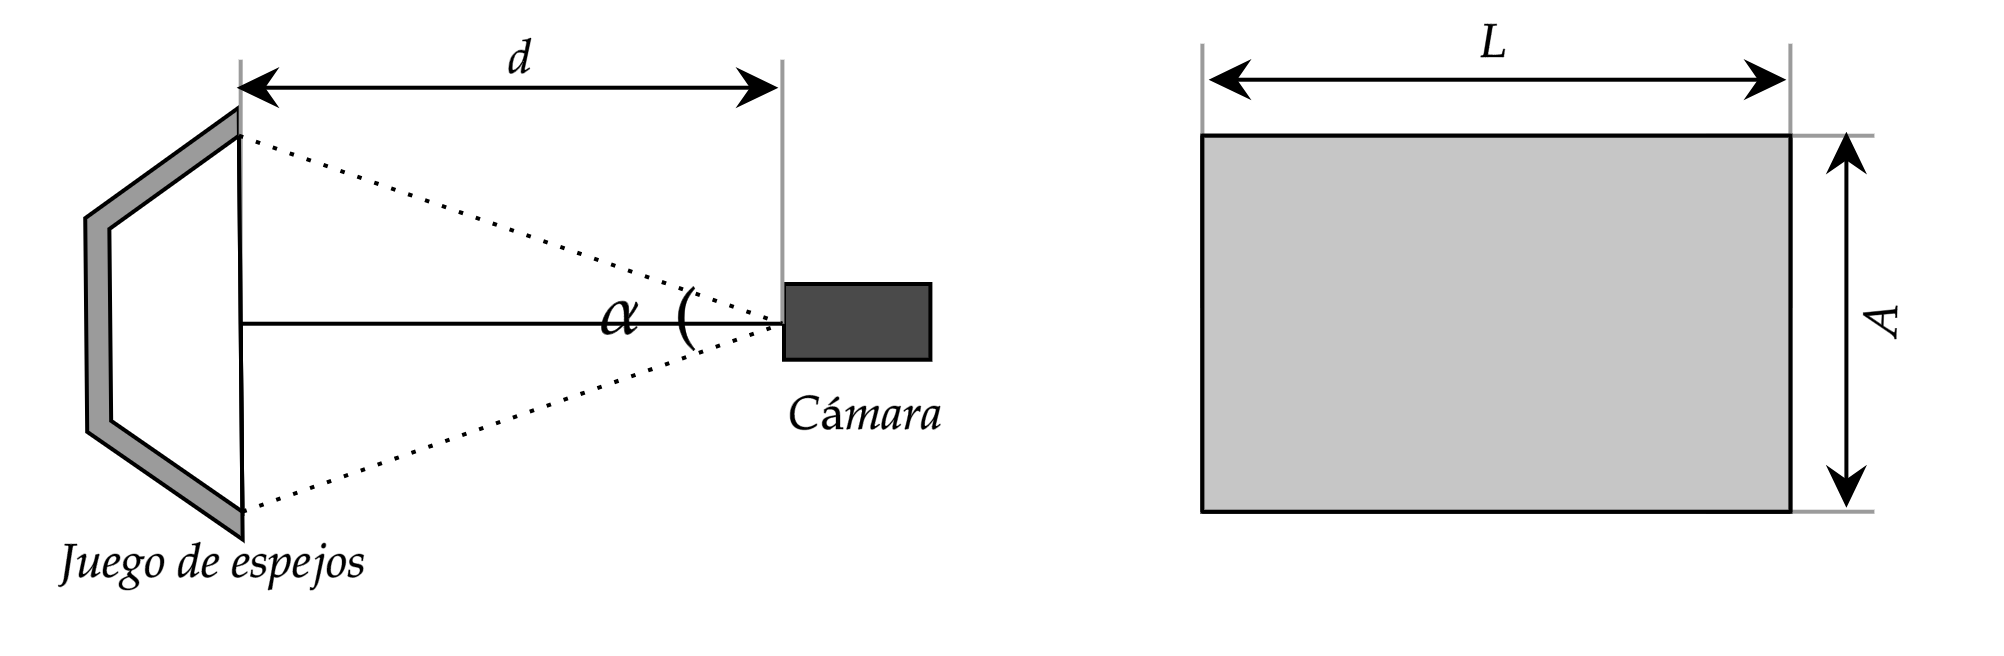
\includegraphics[width=1\textwidth]{chapter5/distancia entre juego de espejos y camara estereo.png}
		\caption{Distancia entre juego de espejos y cámara estéreo}
		\begin{myflushleftportland}
			Fuente: Elaboración propia.
		\end{myflushleftportland}
		\label{fig:distancia entre juego de espejos y camara estereo}
	\end{myfigure}

	De la geometría se obtiene los valores de $\alpha$ y $\beta$, que dependen de las otras variables. El posicionamiento de la cámara ($d$) estéreo estará sujeto a sus valores de HDFV y VDFV como se muestra en la Ecuación \ref{eq:calculo beta de distancia entre espejos y camara estereo} y \ref{eq:calculo alfa de distancia entre espejos y camara estereo}, respectivamente.
		
	\begin{myfigure}[H]
		\centering
		\includegraphics[width=1\textwidth]{chapter5/calculo de distancia entre espejos y camara estereo.png}
		\caption{Cálculo de distancia apropiada para la cámara estéreo}
		\begin{myflushleftportland}
			Fuente: Elaboración propia.
		\end{myflushleftportland}
		\label{fig:calculo de distancia entre espejos y camara estereo}
	\end{myfigure}
	
	\begin{myequation}\label{eq:calculo alfa de distancia entre espejos y camara estereo}
		\begin{split}
			tan(\alpha_{min}/2)&=\frac{A/2}{d}\\
			\alpha_{min}&=2*atan(\frac{A}{2*d})\\
		\end{split}		
	\end{myequation}

	\begin{myequation}\label{eq:calculo beta de distancia entre espejos y camara estereo}
		\begin{split}
			tan(\beta_{min}/2)&=\frac{L/2}{d}\\
			\beta_{min}&=2*atan(\frac{L}{2*d})\\
		\end{split}		
	\end{myequation}


	
	\item \textbf{Selección de cámara estéreo}
	
	El objetivo de la cámara estéreo es la de obtener fotos por determinado periodo de tiempo designado por los algoritmos de procesamiento de imágenes. Con el fin de cumplir el objetivo mencionado deben cumplirse requerimientos técnicos: fotografiar a la trucha con un enfoque aceptable que permita distinguir a la trucha adecuadamente, ángulo de visión horizontal y vertical, resolución, entre otros. En la Figura \ref{fig:diagrama esquematico camara estereo y dependencia de la distancia del objeto} se visualiza un diagrama referencial de una cámara estéreo, con la cuál podemos obtener distancias a partir de dos imágenes. 
	
	\begin{myfigure}[H]
		\centering
		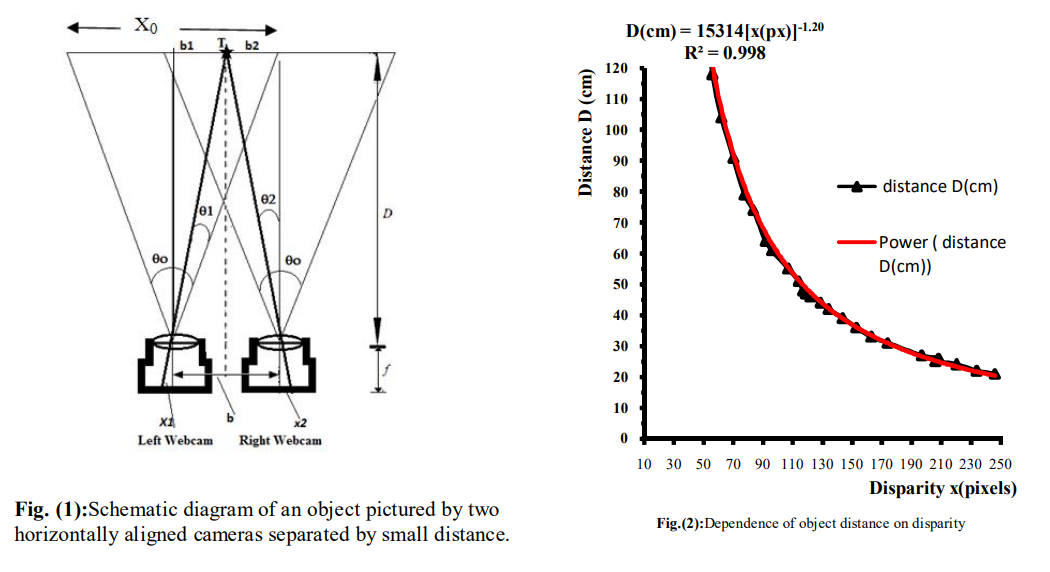
\includegraphics[width=1\textwidth]{chapter5/diagrama esquematico camara estereo y dependencia de la distancia del objeto.png}
		\caption[Diagrama esquemático y dependencia de la distancia del objeto seguido por una cámara estéreo.]{(Izq.) Diagrama esquemático de un objeto representado por dos cámaras alineadas horizontalmente separadas por una pequeña distancia. (Der.) Dependencia de la distancia del objeto en la disparidad.}
		\begin{myflushleftportland}
			Fuente: \cite{Mahammed2013}
		\end{myflushleftportland}
		\label{fig:diagrama esquematico camara estereo y dependencia de la distancia del objeto}
	\end{myfigure}
	
	Por ejemplo, el error realizado en pruebas con vehículos autónomos brindado en \cite{Zaarane2020} se muestra en la Figura \ref{fig:medicion de distancia con distintas distancias}. 
	
	\begin{myfigure}[H]
		\centering
		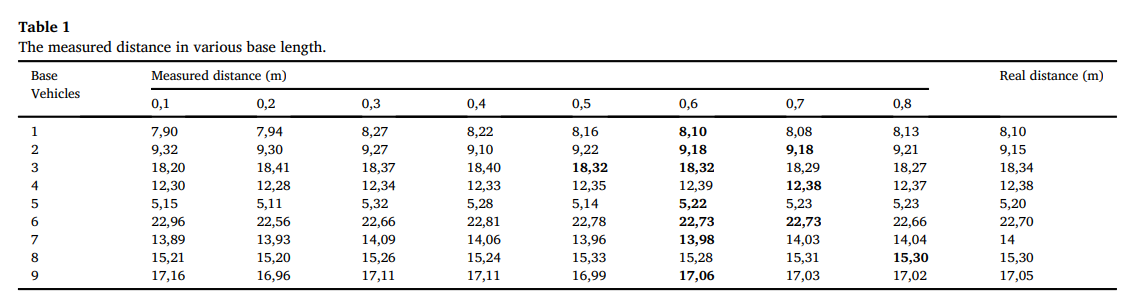
\includegraphics[width=1\textwidth]{chapter5/medicion de distancia con distintas distancias.png}
		\caption{Pruebas de medición con distintas distancias al objeto.}
		\begin{myflushleftportland}
			Fuente: \cite{Zaarane2020}
		\end{myflushleftportland}
		\label{fig:medicion de distancia con distintas distancias}
	\end{myfigure}
		
	%- Tamaño de píxeles requerido \\
	%- Cantidad de frames (80 fps con 3-4L/s) (Falta calcular con lo que hemos calculado 16 cm/s) \\ 
	%- La inclinación hace que el pez no tenga velocidad hacia arriba \\

	
	En la Tabla \ref{tab:tabla comparativa de camaras estereo} se muestra tanto los requerimientos mínimos como las cámaras estéreo candidatas para el sistema. El cálculo mencionado en la sección anterior se calcula luego de escoger una de entre las tres opciones mostradas.
	
	\begin{savenotes}
	\begin{mytable}[H]
		\centering
		\caption{Tabla comparativa de cámaras estéreo.}
		\label{tab:tabla comparativa de camaras estereo}
		\begin{tabular}{l|c|c|c|c|}
			\cline{2-5}
			\multicolumn{1}{c|}{\textbf{}}            & \textbf{\begin{tabular}[c]{@{}c@{}}Requisitos\\ mínimos\end{tabular}} & 
			\multicolumn{1}{|l|}{				
				\begin{minipage}{\mythirdmaxsizeofcontenttable}
					\begin{myflushcenter}
						\textbf{OAK-D}
					\end{myflushcenter}
				\end{minipage}
			}&
			\multicolumn{1}{|l|}{				
				\begin{minipage}{\mythirdmaxsizeofcontenttable}	
					\begin{myflushcenter}
						\textbf{B0263}
					\end{myflushcenter}
				\end{minipage}
			}&
			\multicolumn{1}{|l|}{				
				\begin{minipage}{\mythirdmaxsizeofcontenttable}	
					\begin{myflushcenter}
						\textbf{B0204}
					\end{myflushcenter}
				\end{minipage}
			}  \\ \hline
			\multicolumn{1}{|l|}{\textbf{Figura}} & - 
			&		  
			\begin{minipage}{\mythirdmaxsizeofcontenttable}
				\centering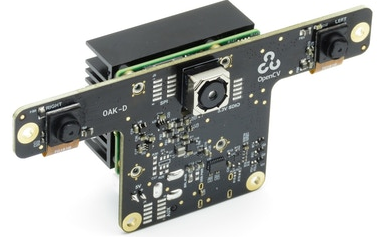
\includegraphics[width=\mythirdmaxsizeimageinsidetable]{chapter5/tablas comparativas/camara estereo 1.png} \\ 
				%\begin{myflushcenter}
				%	{\footnotesize Nombre imagen}
				%\end{myflushcenter}
			\end{minipage}
			&		  
			\begin{minipage}{\mythirdmaxsizeofcontenttable}
				\centering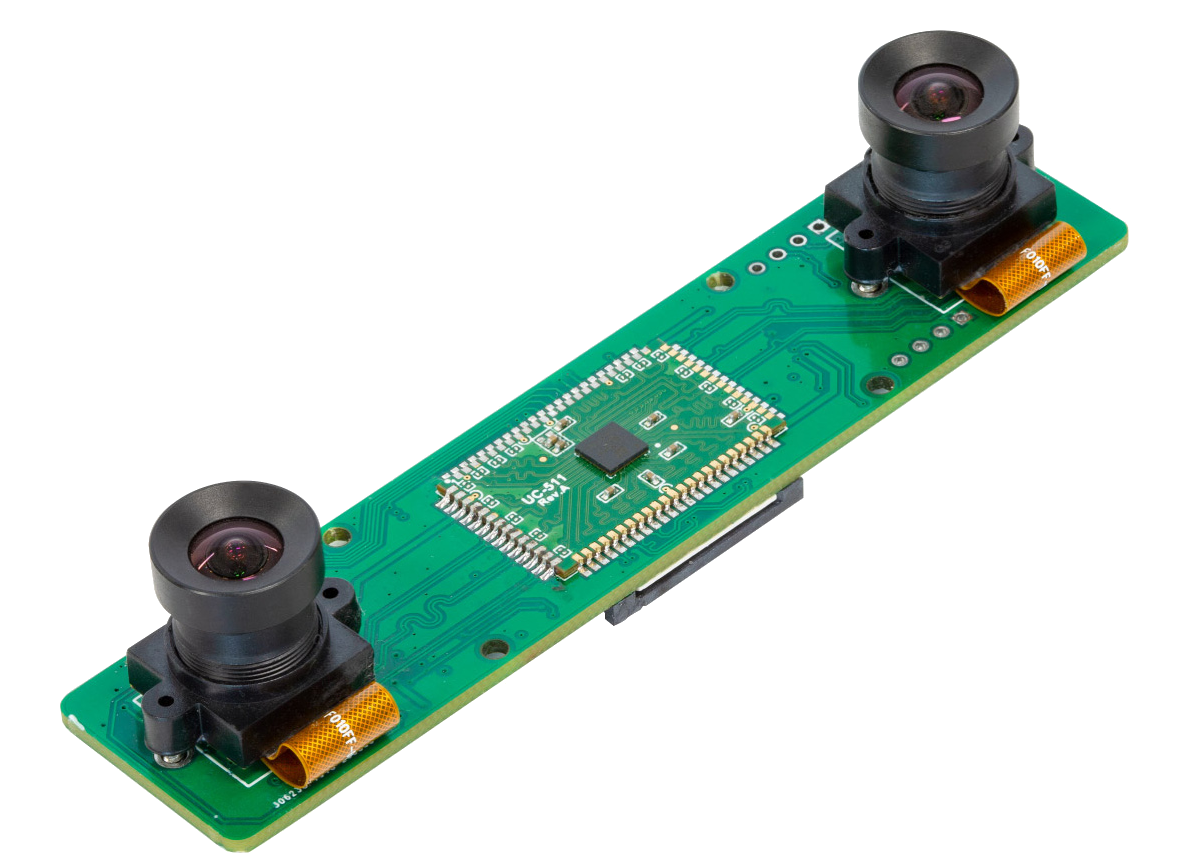
\includegraphics[width=\mythirdmaxsizeimageinsidetable]{chapter5/tablas comparativas/camara estereo 2.png} \\ 
				%\begin{myflushcenter}
				%	{\footnotesize Nombre imagen}
				%\end{myflushcenter}
			\end{minipage}
			&  
			\begin{minipage}{\mythirdmaxsizeofcontenttable}
				\centering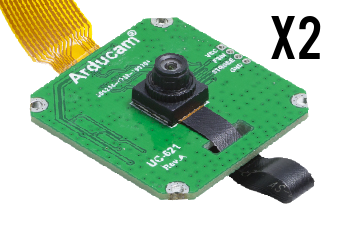
\includegraphics[width=\mythirdmaxsizeimageinsidetable]{chapter5/tablas comparativas/camara estereo 3.png} \\ 
				%\begin{myflushcenter}
				%	{\footnotesize Nombre imagen}
				%\end{myflushcenter}
			\end{minipage}\\ \hline
			\multicolumn{1}{|l|}{
				\begin{minipage}{\myforthmaxsizeofcontenttable}	
					\textbf{Fabricante}
				\end{minipage}
			} & - & OpenCV & ArduCam & ArduCam \\ \hline
			\multicolumn{1}{|l|}{
				\begin{minipage}{\myforthmaxsizeofcontenttable}	
					\textbf{Sensor óptico}
				\end{minipage}
			} & - & OV9282 & OV9281 & OV2311 \\ \hline
			\multicolumn{1}{|l|}{
				\begin{minipage}{\myforthmaxsizeofcontenttable}	
					\textbf{Tipo de obturador}
				\end{minipage}
			} & 
			\begin{minipage}{\mythirdmaxsizeofcontenttable}\begin{myflushcenter}
				Global sincronizado 
			\end{myflushcenter}\end{minipage} & 
			\begin{minipage}{\mythirdmaxsizeofcontenttable}\begin{myflushcenter}
				Global sincronizado 
			\end{myflushcenter}\end{minipage} &
			\begin{minipage}{\mythirdmaxsizeofcontenttable}\begin{myflushcenter}
				Global sincronizado 
			\end{myflushcenter}\end{minipage}&
			\begin{minipage}{\mythirdmaxsizeofcontenttable}\begin{myflushcenter}
				Global dual 
			\end{myflushcenter}\end{minipage} \\ \hline
			\multicolumn{1}{|l|}{
				\begin{minipage}{\myforthmaxsizeofcontenttable}	
					\textbf{Escala de colores}
				\end{minipage}
			} & - & RGB & B/N & B/N \\ \hline
			\multicolumn{1}{|l|}{
				\begin{minipage}{\myforthmaxsizeofcontenttable}	
					\textbf{Resolución}
				\end{minipage}
			} & 0.5MP & 
			\begin{minipage}{\mythirdmaxsizeofcontenttable}\begin{myflushcenter}
					1MP (1280× 800 $px/3{\mu}m$)
			\end{myflushcenter}\end{minipage} & 
			\begin{minipage}{\mythirdmaxsizeofcontenttable}\begin{myflushcenter}
					1MP (1280× 800 $px/3{\mu}m$)
			\end{myflushcenter}\end{minipage} & 
			\begin{minipage}{\mythirdmaxsizeofcontenttable}\begin{myflushcenter}
					2MP (1600x 1300 $px/3{\mu}m$)
			\end{myflushcenter}\end{minipage} \\ \hline
			\multicolumn{1}{|l|}{
				\begin{minipage}{\myforthmaxsizeofcontenttable}	
					\textbf{Frames por segundo ($FPS$)}
				\end{minipage}
			} & 60 % NECESITO MÁS DE 80
			& 120 & 60 & 60 \\ \hline
			\multicolumn{1}{|l|}{
				\begin{minipage}{\myforthmaxsizeofcontenttable}	
					\textbf{Tamaño de lente ('')}
				\end{minipage}
			} & Independiente & 1/2.3 & 1/4 & 1/2.9 \\ \hline
			\multicolumn{1}{|l|}{
				\begin{minipage}{\myforthmaxsizeofcontenttable}	
					\textbf{Enfoque ($mm.$)}
				\end{minipage}
			} & - & [196;$\infty$] & [30;$\infty$] & [30;$\infty$] \\ \hline
			\multicolumn{1}{|l|}{
				\begin{minipage}{\myforthmaxsizeofcontenttable}
					\textbf{Campo de visión ° (HFDV,VFDV,DFDV)\footnote{HFDV: Campo de visión horizontal. VFDV: Campo de visión vertical. DFDV: Campo de visión diagonal}}
				\end{minipage}
			} & Adaptable & 71.8, --, 81.0 & 70, 52.1 , -- & 100, 68.2, -- \\ \hline
			\multicolumn{1}{|l|}{
				\begin{minipage}{\myforthmaxsizeofcontenttable}	
					\textbf{Procesamiento gráfico}
				\end{minipage}
			} & - & MA2085 VPU\footnote{Movidius™ Myriad™ VPU. \href{https://www.intel.com/content/www/us/en/products/processors/movidius-vpu/movidius-myriad-x.html}{Enlace a unidad de procesamiento de visión.}} & 
			\begin{minipage}{\mythirdmaxsizeofcontenttable}\begin{myflushcenter}
				Jetson Nano o Xavier NX
			\end{myflushcenter}\end{minipage}
		 	& \begin{minipage}{\mythirdmaxsizeofcontenttable}\begin{myflushcenter}
		 			Raspberry Pi 3
		 	\end{myflushcenter}\end{minipage} \\ \hline 
		 	\multicolumn{1}{|l|}{
		 		\begin{minipage}{\myforthmaxsizeofcontenttable}	
		 			\textbf{Temperatura operativa}
		 		\end{minipage}
		 	} & [-10;50] & [-30;60] & [-30;85] & [-30;85] \\ \hline
			\multicolumn{1}{|l|}{
				\begin{minipage}{\myforthmaxsizeofcontenttable}	
					\textbf{Soporte IA\footnote{Chips diseñados y optimizados para procesar detección de objetos mediante redes neuronales.}}
				\end{minipage}
			} & - & Sí & Sí & No \\ \hline
			\multicolumn{1}{|l|}{
				\begin{minipage}{\myforthmaxsizeofcontenttable}	
					\textbf{Consumo de energía ($W$)}
				\end{minipage}
			} & <10 & $\approx6$ & - & - \\ \hline
			\multicolumn{1}{|l|}{
				\begin{minipage}{\myforthmaxsizeofcontenttable}	
					\textbf{Precio (S/)}
				\end{minipage}
			} & <1000 & 475.41 & 358.97 & 717.28 \\ \hline
		\end{tabular}
		\begin{flushleft}	
			Fuente: OpenCV, ArduCam y elaboración propia. Hoja de datos técnico (\textit{Datasheet}) en el Anexo.\\
			Tasa de cambio de USD a PEN: S/ 3.59.
		\end{flushleft}
	\end{mytable}
	\end{savenotes}
	
	\textcolor{blue}{[BORRADOR] Decicisión de qué actuador será escogido y por qué en base a las características mencionadas [/BORRADOR]}
	
	\item \textbf{Selección de cámara simple}
	
	La cámara simple tiene como función verificar la correcta trayectoria de las truchas en el mecanismo de distribución hacia las respectivas jaulas flotantes. Los requerimientos técnicos se presentan en la Tabla \ref{tab:tabla comparativa de camaras simples} así como las principales características de cada una.
	
	\begin{savenotes}
		\begin{mytable}[H]
			\centering
			\caption{Tabla comparativa de cámaras.}
			\label{tab:tabla comparativa de camaras simples}
			\begin{tabular}{l|c|c|c|c|}
				\cline{2-5}
				\multicolumn{1}{c|}{\textbf{}}            & \textbf{\begin{tabular}[c]{@{}c@{}}Requisitos\\ mínimos\end{tabular}} & 
				\multicolumn{1}{|l|}{				
					\begin{minipage}{\mythirdmaxsizeofcontenttable}
						\begin{myflushcenter}
							\textbf{B0249}
						\end{myflushcenter}
					\end{minipage}
				}&
				\multicolumn{1}{|l|}{				
					\begin{minipage}{\mythirdmaxsizeofcontenttable}	
						\begin{myflushcenter}
							\textbf{Alvium 1800 U-500m}
						\end{myflushcenter}
					\end{minipage}
				}&
				\multicolumn{1}{|l|}{				
					\begin{minipage}{\mythirdmaxsizeofcontenttable}	
						\begin{myflushcenter}
							\textbf{CMT-8MP- IMX219M366}
						\end{myflushcenter}
					\end{minipage}
				}  \\ \hline
				\multicolumn{1}{|l|}{\textbf{Figura}} & - 
				&		  
				\begin{minipage}{\mythirdmaxsizeofcontenttable}
					\centering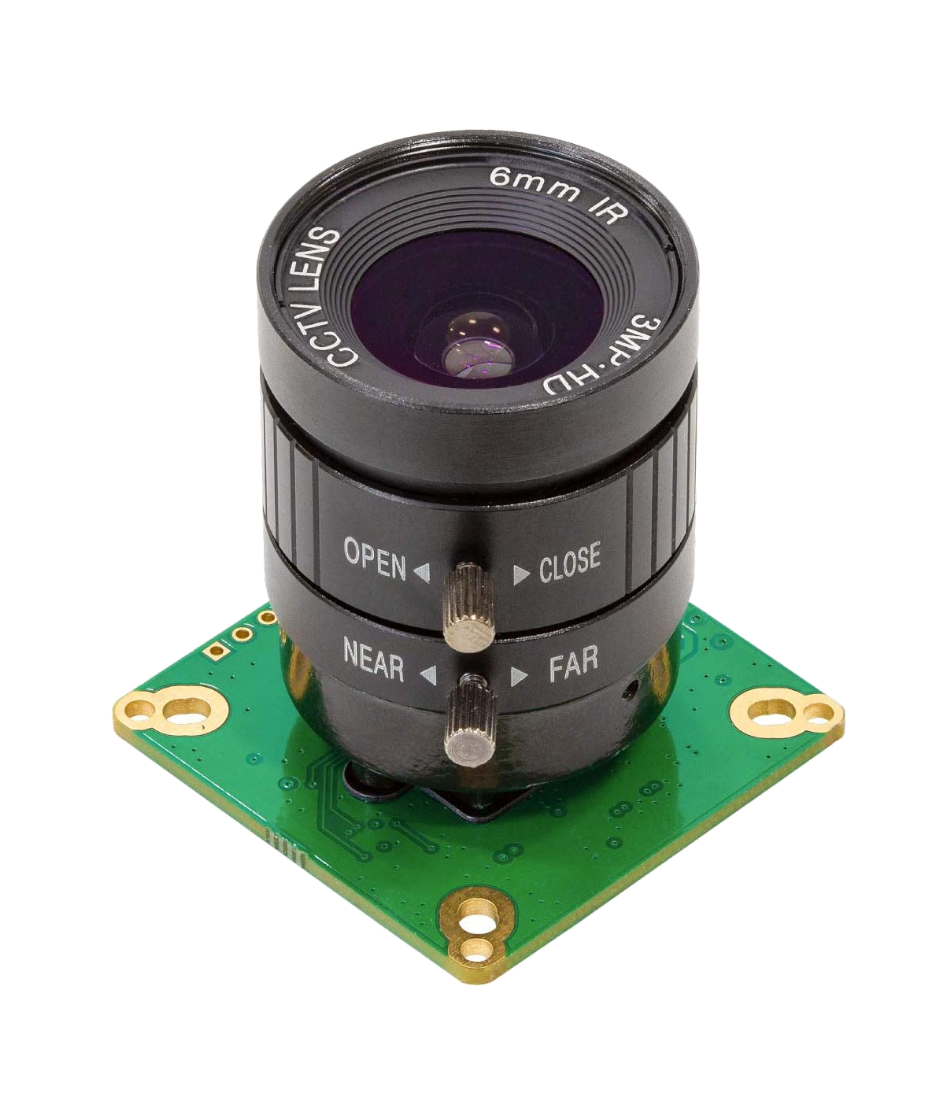
\includegraphics[width=\mythirdmaxsizeimageinsidetable]{chapter5/tablas comparativas/camara simple 1.png} \\ 
					%\begin{myflushcenter}
					%	{\footnotesize Nombre imagen}
					%\end{myflushcenter}
				\end{minipage}
				&		  
				\begin{minipage}{\mythirdmaxsizeofcontenttable}
					\centering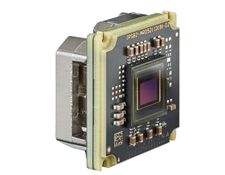
\includegraphics[width=\mythirdmaxsizeimageinsidetable]{chapter5/tablas comparativas/camara simple 2.png} \\ 
					%\begin{myflushcenter}
					%	{\footnotesize Nombre imagen}
					%\end{myflushcenter}
				\end{minipage}
				&  
				\begin{minipage}{\mythirdmaxsizeofcontenttable}
					\centering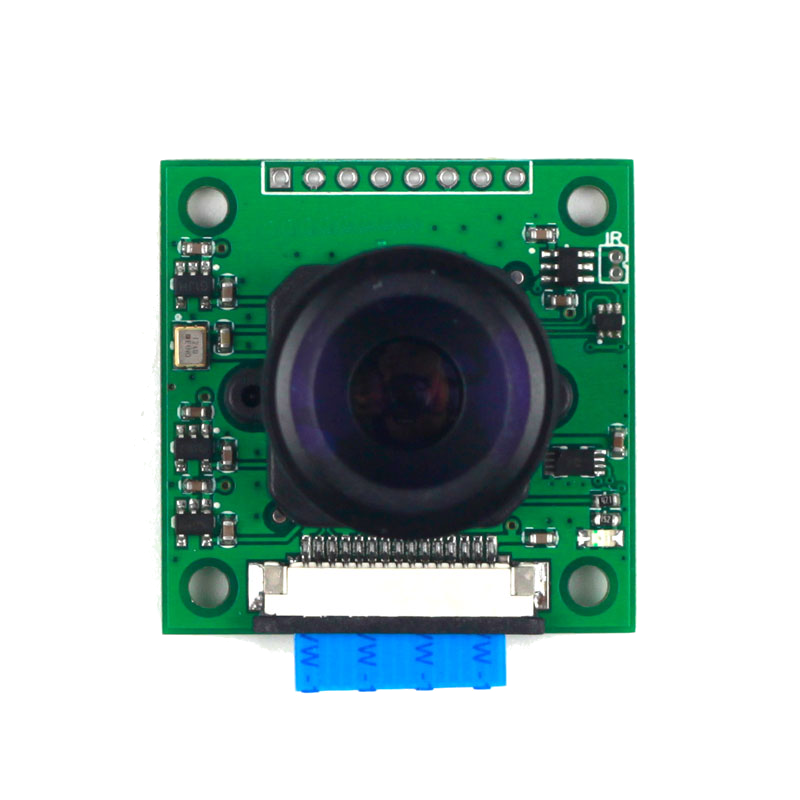
\includegraphics[width=\mythirdmaxsizeimageinsidetable]{chapter5/tablas comparativas/camara simple 3.png} \\ 
					%\begin{myflushcenter}
					%	{\footnotesize Nombre imagen}
					%\end{myflushcenter}
				\end{minipage}\\ \hline
				\multicolumn{1}{|l|}{
					\begin{minipage}{\myforthmaxsizeofcontenttable}	
						\textbf{Fabricante}
					\end{minipage}
				} & - & ArduCam & Allied Vision & ArduCam \\ \hline
				\multicolumn{1}{|l|}{
					\begin{minipage}{\myforthmaxsizeofcontenttable}	
						\textbf{Sensor óptico}
					\end{minipage}
				} & - & IMX477  & 
				\begin{minipage}{\mythirdmaxsizeofcontenttable}\begin{myflushcenter}
						ON Semi AR0521SR
				\end{myflushcenter}\end{minipage} & IMX219 \\ \hline
				\multicolumn{1}{|l|}{
					\begin{minipage}{\myforthmaxsizeofcontenttable}	
						\textbf{Tipo de obturador}
					\end{minipage}
				} & 
				\begin{minipage}{\mythirdmaxsizeofcontenttable}\begin{myflushcenter}
						- 
				\end{myflushcenter}\end{minipage} & 
				\begin{minipage}{\mythirdmaxsizeofcontenttable}\begin{myflushcenter}
						Global
				\end{myflushcenter}\end{minipage} &
				\begin{minipage}{\mythirdmaxsizeofcontenttable}\begin{myflushcenter}
						Rolling 
				\end{myflushcenter}\end{minipage}&
				\begin{minipage}{\mythirdmaxsizeofcontenttable}\begin{myflushcenter}
						Rolling 
				\end{myflushcenter}\end{minipage} \\ \hline
				\multicolumn{1}{|l|}{
					\begin{minipage}{\myforthmaxsizeofcontenttable}	
						\textbf{Escala de colores}
					\end{minipage}
				} & - & RGB & B/N & RGB \\ \hline
				\multicolumn{1}{|l|}{
				\begin{minipage}{\myforthmaxsizeofcontenttable}	
					\textbf{Resolución}
				\end{minipage}
				} & 0.5MP & 
				\begin{minipage}{\mythirdmaxsizeofcontenttable}\begin{myflushcenter}
					12.3MP (4056× 3040 $px/1.55{\mu}m$)
				\end{myflushcenter}\end{minipage} & 
				\begin{minipage}{\mythirdmaxsizeofcontenttable}\begin{myflushcenter}
					5MP (2592x 1944 $px/2.2{\mu}m$)
				\end{myflushcenter}\end{minipage} & 
				\begin{minipage}{\mythirdmaxsizeofcontenttable}\begin{myflushcenter}
					8MP (3280x 2464 $px/1.12{\mu}m$)
				\end{myflushcenter}\end{minipage} \\ \hline
				\multicolumn{1}{|l|}{
				\begin{minipage}{\myforthmaxsizeofcontenttable}	
					\textbf{Frames por segundo ($FPS$)}
				\end{minipage}
				} & 40 % NECESITO MÁS DE 80
				& 60 & 67 & 720p60 \\ \hline
				\multicolumn{1}{|l|}{
				\begin{minipage}{\myforthmaxsizeofcontenttable}	
					\textbf{Tamaño de lente ('')}
				\end{minipage}
				} & Independiente & 1/2.3 & 1/2.5 & 1/4 \\ \hline
				\multicolumn{1}{|l|}{
				\begin{minipage}{\myforthmaxsizeofcontenttable}
					\textbf{Campo de visión ° (HFDV,VFDV,DFDV)\footnote{HFDV: Campo de visión horizontal. VFDV: Campo de visión vertical. DFDV: Campo de visión diagonal}}
				\end{minipage}
				} & Adaptable & 65.0, --, -- & -- & 70, 70, -- \\ \hline
				\multicolumn{1}{|l|}{
				\begin{minipage}{\myforthmaxsizeofcontenttable}	
					\textbf{Procesamiento gráfico}
				\end{minipage}
				} & - & 
				\begin{minipage}{\mythirdmaxsizeofcontenttable}\begin{myflushcenter}
					Jetson Nano o Xavier NX
				\end{myflushcenter}\end{minipage} & 
				\begin{minipage}{\mythirdmaxsizeofcontenttable}\begin{myflushcenter}
					Jetson Nano o Xavier NX
				\end{myflushcenter}\end{minipage}&
				\begin{minipage}{\mythirdmaxsizeofcontenttable}\begin{myflushcenter}
					Raspberry Pi
				\end{myflushcenter}\end{minipage} \\ \hline 
				\multicolumn{1}{|l|}{
				\begin{minipage}{\myforthmaxsizeofcontenttable}	
					\textbf{Temperatura operativa}
				\end{minipage}
				} & [-10;50] & [-20;60] & [5;80] & [-20;70] \\ \hline
				\multicolumn{1}{|l|}{
				\begin{minipage}{\myforthmaxsizeofcontenttable}	
					\textbf{Consumo de energía ($W$)}
				\end{minipage}
				} & <5 & - & [$\approx$2.2;$\approx$2.4] & - \\ \hline
				\multicolumn{1}{|l|}{
				\begin{minipage}{\myforthmaxsizeofcontenttable}	
					\textbf{Precio (S/)}
				\end{minipage}
				} & <500 & 196.81 & 595.7 & 717.28 \\ \hline
				\end{tabular}
			\begin{flushleft}	
				Fuente: Allied Vision, ArduCam y elaboración propia. Hoja de datos técnico (\textit{Datasheet}) en el Anexo.\\
				Tasa de cambio de USD a PEN: S/ 3.59.
			\end{flushleft}
		\end{mytable}
	\end{savenotes}
	
	\textcolor{blue}{[BORRADOR] Decicisión de qué actuador será escogido y por qué en base a las características mencionadas [/BORRADOR]}
	
	
	
\end{itemize}



%% NUEVO SUBSECCION X.X.X.X
\subsubsection{Selección de iluminación adecuada} 


Dolor sed viverra ipsum nunc aliquet bibendum. Euismod in pellentesque massa placerat. Et malesuada fames ac turpis egestas sed tempus urna. Euismod elementum nisi quis eleifend quam adipiscing vitae proin.

%% NUEVO SUBSECCION X.X.X.X
\subsubsection{Selección de led de alta potencia}

El propósito de los leds de alta potencia es iluminar la zona en la que se realiza la captura de imágenes para detectar truchas y procesarlas. El uso de una led adecuado puede mejorar el rendimiento de la cámara. En la Figura \ref{fig:iluminacion opciones} se muestra las opciones de iluminación que se consideraron, resultando el uso de dos tiras de leds adecuadas para el sistema.

% EN LA CARPETA IMAGENES ESTAN TODA LAS IMAGENES BASE
\begin{myfigure}[H]
	\centering
	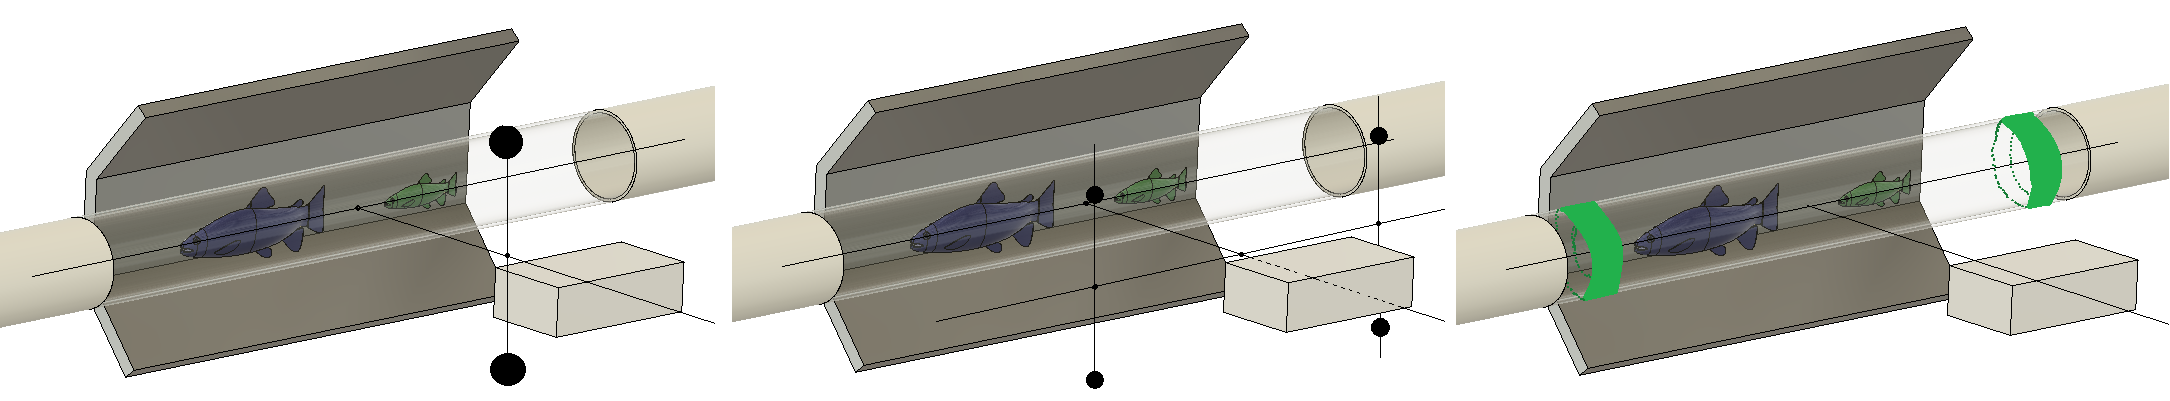
\includegraphics[width=1\textwidth]{chapter5/iluminacion opciones.png}
	\caption[Opciones de posicionamiento de iluminación.]{(Izq.) Iluminación con dos leds frente al sistema. (Cen.) Iluminación con cuatro leds frente al sistema. (Der.) Iluminación con dos tiras leds.}
	\begin{myflushleftportland}
		Fuente: Elaboración propia.
	\end{myflushleftportland}
	\label{fig:iluminacion opciones}
\end{myfigure}


La selección de una iluminación adecuada es tan importante como la selección de los otros componentes del subsistema: la ausencia de una iluminación adecuada puede degradar el rendimiento de los algoritmos, así como los de obtención de fotografías en la cámara estéreo debido al tiempo de exposición necesario por fotografía.

\begin{myequation}\label{eq:calculo de led de alta potencia}
	\begin{split}
		Iluminación_{necesaria}&=1000 %(lumenes)
	\end{split}		
\end{myequation}

En la Tabla XX se muestra una tabla técnica comparativa.

\begin{myfigure}[H]
	\centering
	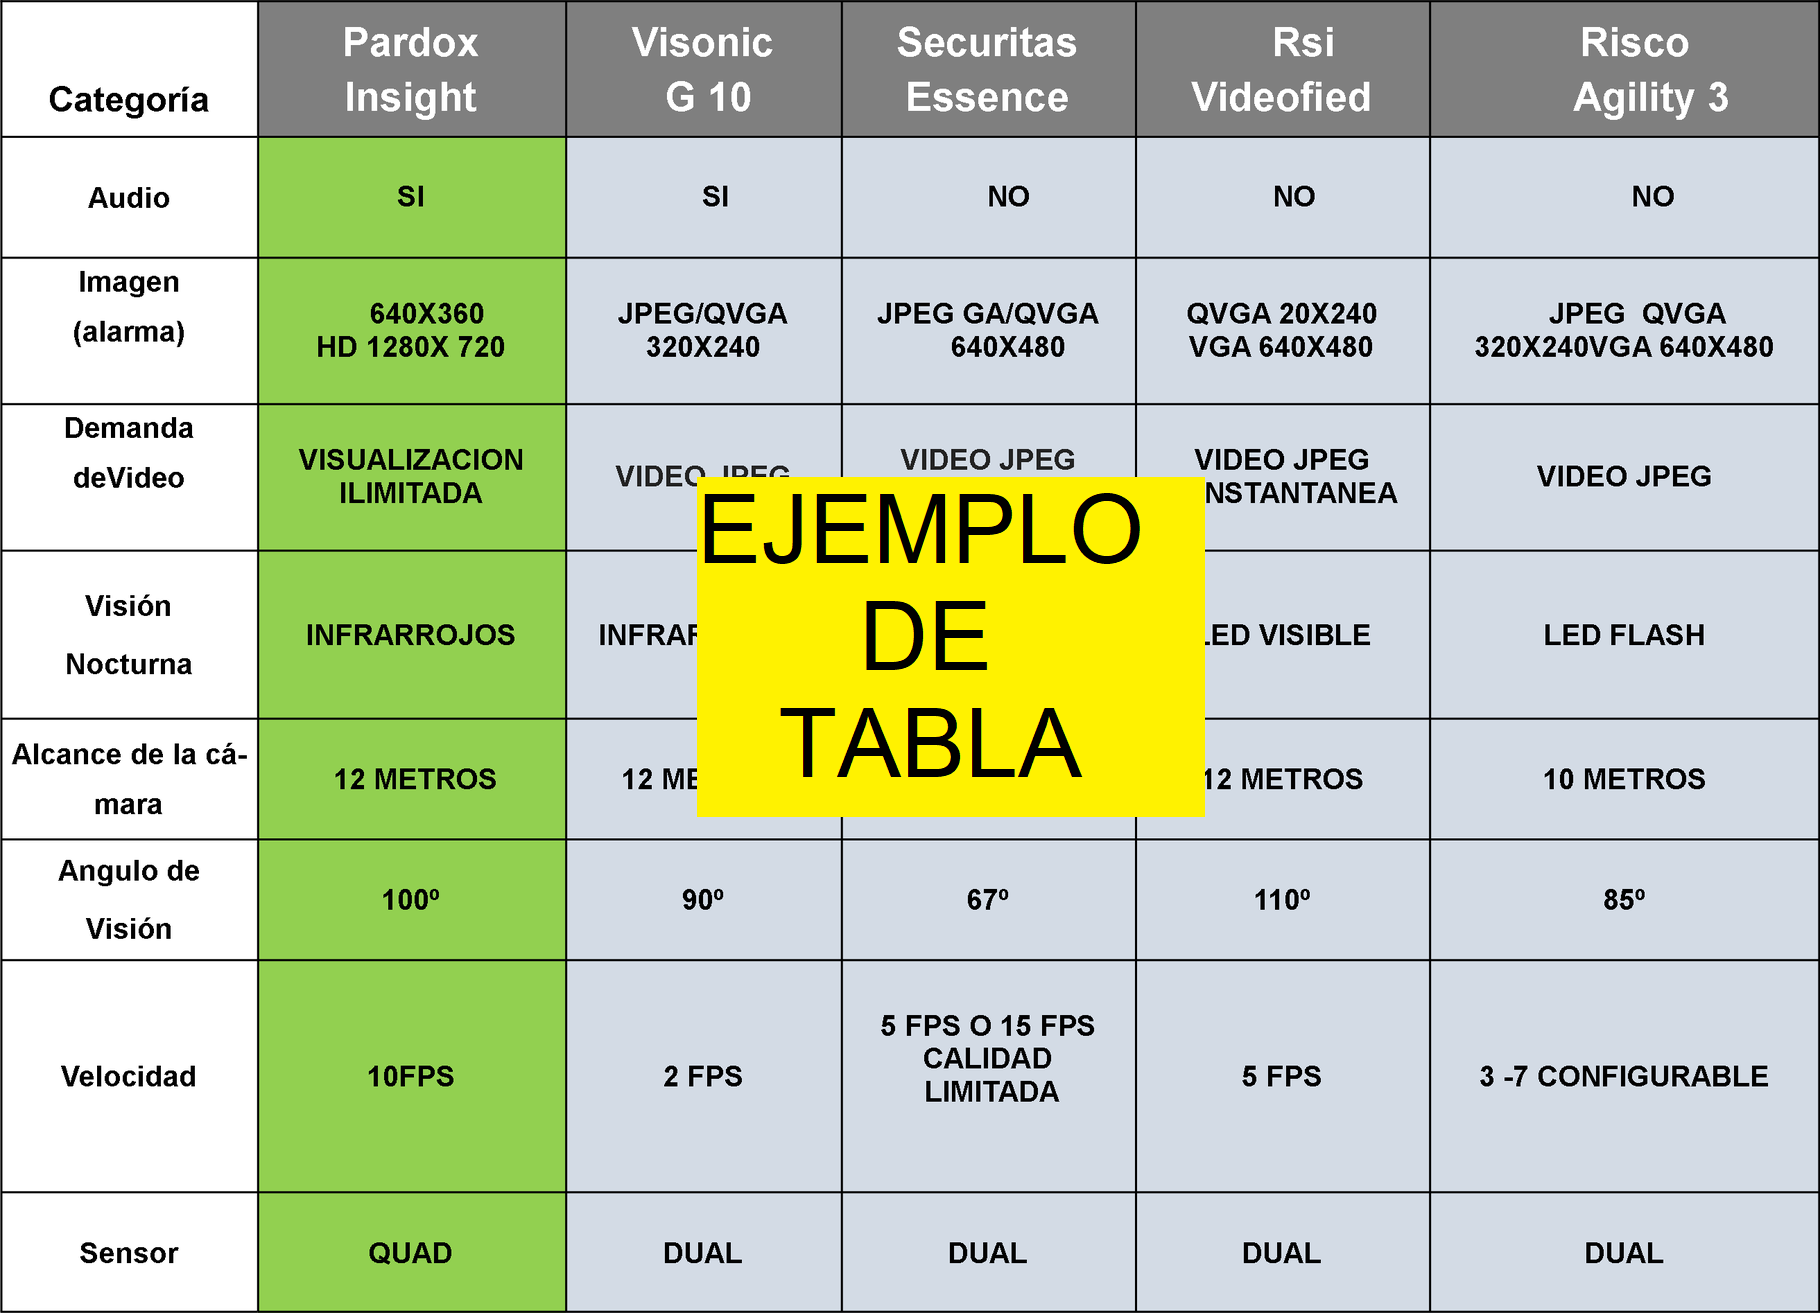
\includegraphics[width=0.85\textwidth]{chapter5/ejemplo de tabla.png}
	\caption{Ejemplo de tabla}
	\begin{myflushleftportland}
		Fuente: Elaboración propia.
	\end{myflushleftportland}
	\label{fig:ejemplo de tabla}
\end{myfigure}

%% NUEVO SUBSECCION X.X.X.X
\subsubsection{Selección de algoritmos}
\label{sssec:seleccion de algoritmos}

Los algoritmos tienen como objetivo contar y clasificar truchas. Dichos algoritmos son evaluados en la Tabla XXX mediante una comparación técnica en cuanto a diversos puntos: tiempo de respuesta, costo de hardware requerido, consumo eléctrico del hardware, ......

- NN: YOLO,YOLOv2,YOLOv3,YOLOv4,YOLOv5 \\
- NN: CNN - Fish segmentation \\
- Segmentación por características \\

Referencia a todas las versiones de YOLO. YOLO \cite{Redmon2016}, YOLO v2.0 \cite{Redmon2017}, YOLO v3.0 \cite{Redmon2018}, YOLO v4.0 \cite{Solawetz2020}, YOLO v5.0 \cite{bochkovskiy2020yolov4}.


\begin{itemize}
	
	\item \textbf{Selección de algoritmo contador de truchas} 
	
	Lorem ipsum dolor sit amet, consectetur adipiscing elit, sed do eiusmod tempor incididunt ut labore et dolore magna aliqua. Lacus sed turpis tincidunt id aliquet. Nunc aliquet bibendum enim facilisis gravida neque convallis a. Ut tellus elementum sagittis vitae et leo duis ut diam. Dolor sit amet consectetur adipiscing elit ut aliquam purus sit.
	
	\begin{myfigure}[H]
		\centering
		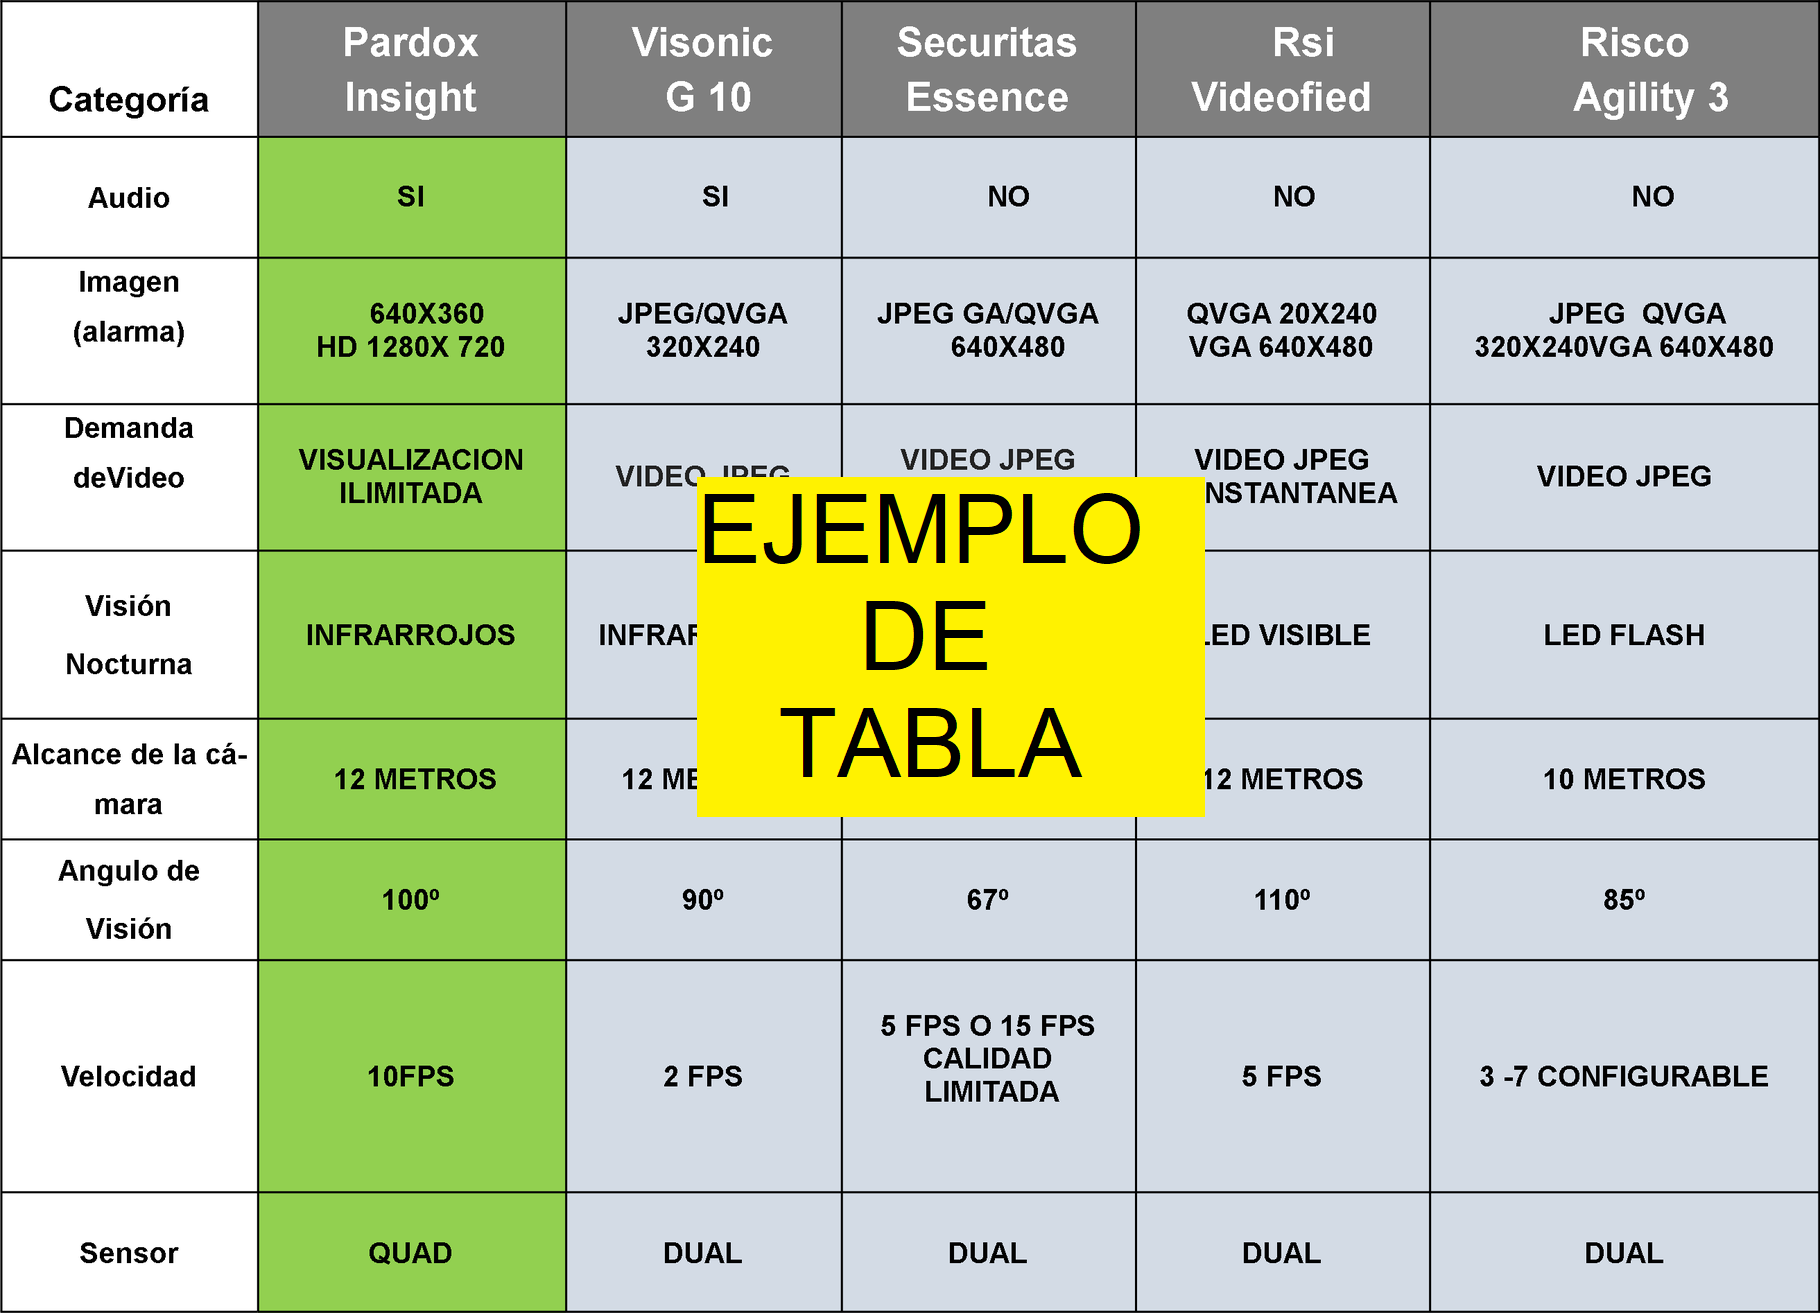
\includegraphics[width=0.85\textwidth]{chapter5/ejemplo de tabla.png}
		\caption{Ejemplo de tabla}
		\begin{myflushleftportland}
			Fuente: Elaboración propia.
		\end{myflushleftportland}
		\label{fig:ejemplo de tabla}
	\end{myfigure}

	Nunc aliquet bibendum enim facilisis gravida neque convallis a. Ut tellus elementum sagittis vitae et leo duis ut diam. Dolor sit amet consectetur adipiscing elit ut aliquam purus sit.
	
	\item \textbf{Selección de algoritmo clasificador de truchas} 
	
	Lorem ipsum dolor sit amet, consectetur adipiscing elit, sed do eiusmod tempor incididunt ut labore et dolore magna aliqua. Lacus sed turpis tincidunt id aliquet. Nunc aliquet bibendum enim facilisis gravida neque convallis a. Ut tellus elementum sagittis vitae et leo duis ut diam. Dolor sit amet consectetur adipiscing elit ut aliquam purus sit.
	
	\begin{myfigure}[H]
		\centering
		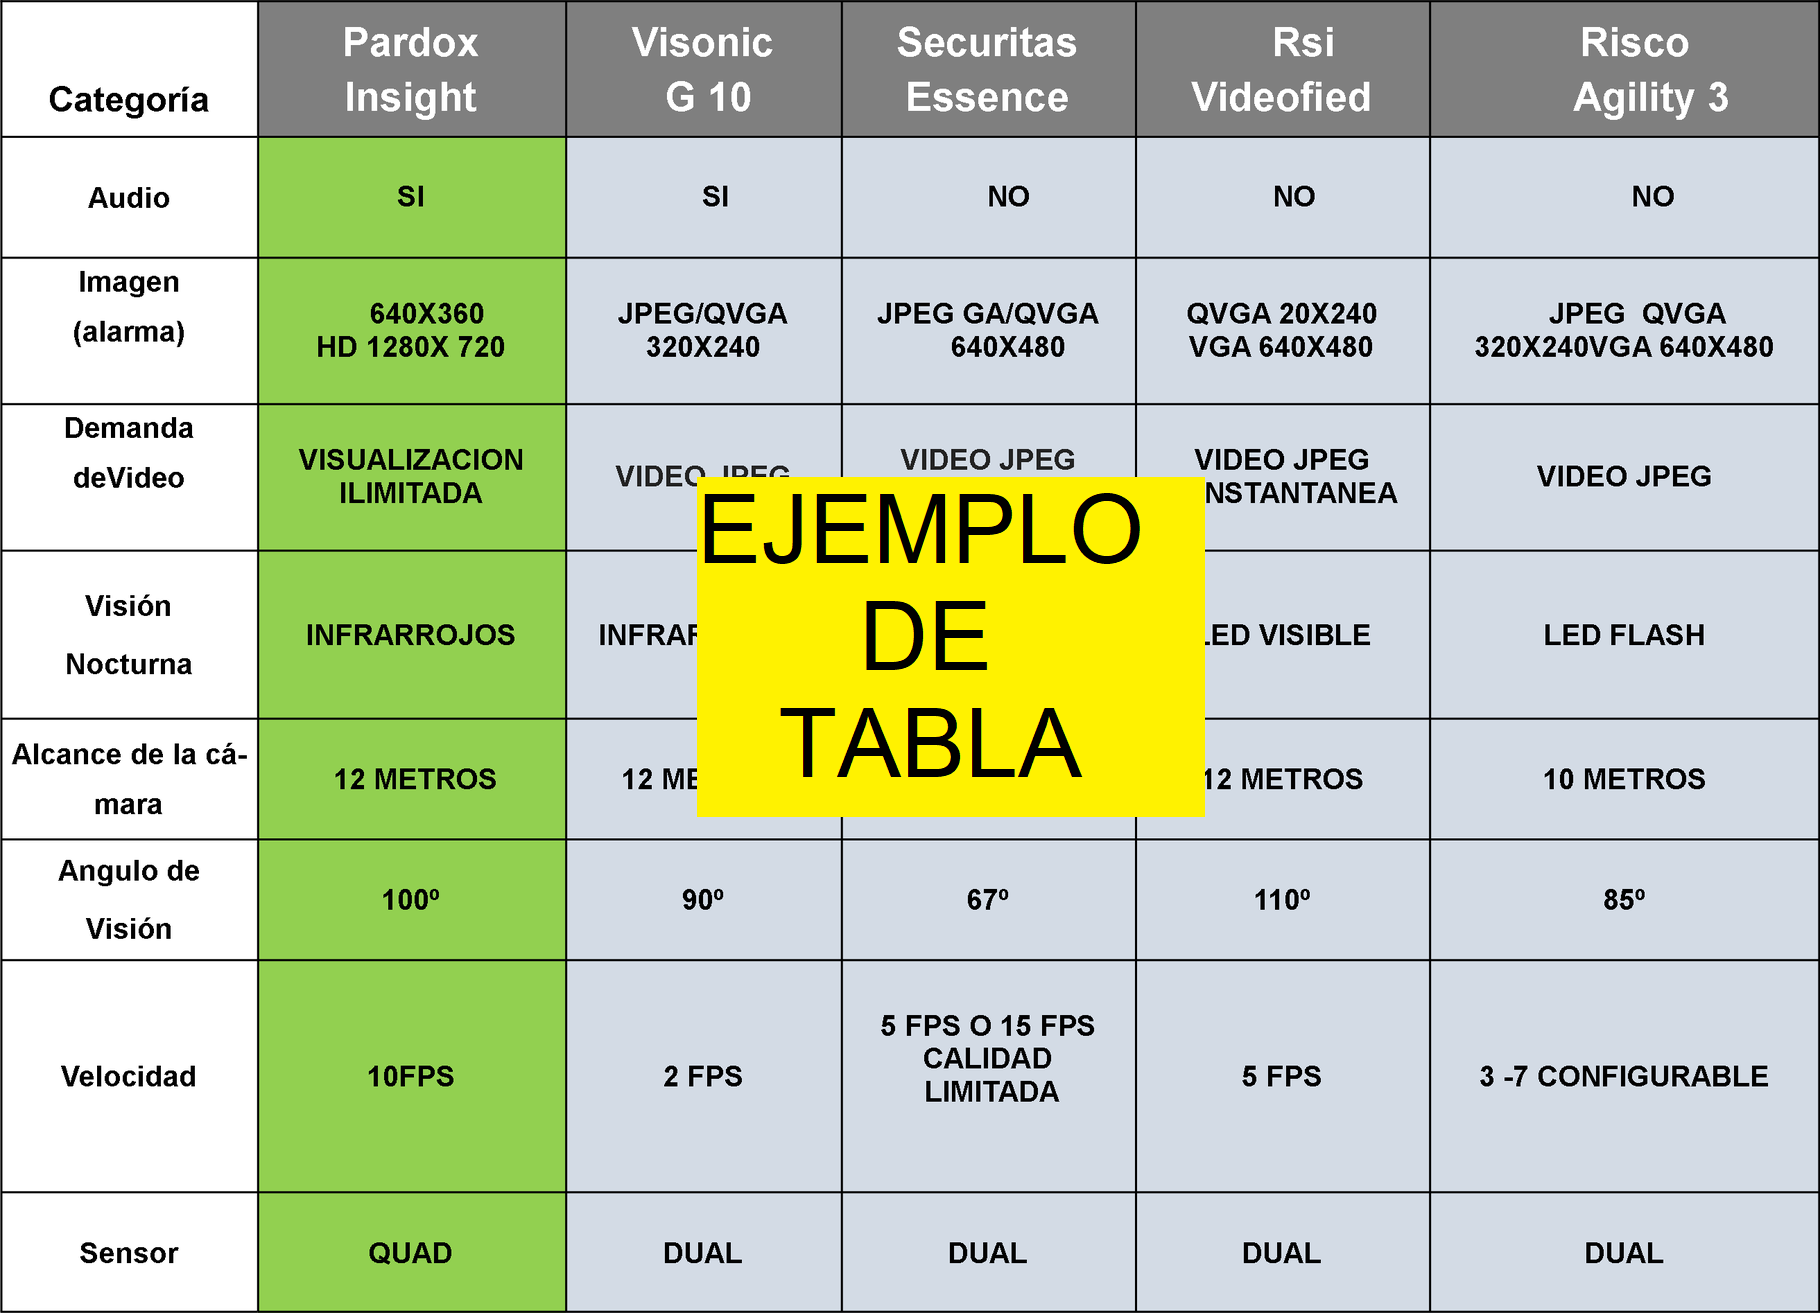
\includegraphics[width=0.85\textwidth]{chapter5/ejemplo de tabla.png}
		\caption{Ejemplo de tabla}
		\begin{myflushleftportland}
			Fuente: Elaboración propia.
		\end{myflushleftportland}
		\label{fig:ejemplo de tabla}
	\end{myfigure}
	
	Nunc aliquet bibendum enim facilisis gravida neque convallis a. Ut tellus elementum sagittis vitae et leo duis ut diam. Dolor sit amet consectetur adipiscing elit ut aliquam purus sit.
	
\end{itemize}

%% NUEVA SECCIÓN X.X.X
\subsection{Subsistema de suministro de energía}
\label{ssec:subsistema de suministro de energia}

El sistema debe suministrar energía a los diversos mecanismos electrónicos, sistemas de control y actuadores necesarios para que la máquina funcione de manera apropiada. Este subsistema debe cumplir diversos requerimientos: estar herméticamente aislado a la entrada de agua, ........\\
En los siguientes párrafos se analizaran a detalle: la selección de la batería, la selección de la fuente de alimentación, la selección de transformadores, la selección de fuentes switching, el diagrama esquemático y el diagrama eléctrico.



%% NUEVO SUBSECCION X.X.X.X
\subsubsection{Selección de la batería} 

Ut tellus elementum sagittis vitae et leo duis ut diam. Dolor sit amet consectetur adipiscing elit ut aliquam purus sit.  Dolor sit amet consectetur adipiscing elit ut aliquam purus sit. las elementum sagittis vitae et.


%% NUEVO SUBSECCION X.X.X.X
\subsubsection{Selección de fuente de alimentación} 

Lorem ipsum dolor sit amet, consectetur adipiscing elit, sed do eiusmod tempor incididunt ut labore et dolore magna aliqua. Lacus sed turpis tincidunt id aliquet. Nunc aliquet bibendum enim facilisis gravida neque convallis a. Ut tellus elementum sagittis vitae et leo duis ut diam. Dolor sit amet consectetur adipiscing elit ut aliquam purus sit. Dolor sed viverra ipsum nunc aliquet bibendum. Euismod in pellentesque massa placerat. Et malesuada fames ac turpis egestas sed tempus urna. Euismod elementum nisi quis eleifend quam adipiscing vitae proin. Ornare suspendisse sed nisi lacus sed. Mollis aliquam ut porttitor leo a diam. Varius morbi enim nunc faucibus. Sit amet purus gravida quis blandit turpis cursus in hac.

%% NUEVO SUBSECCION X.X.X.X
\subsubsection{Selección de transformadores rectificadores}

Lorem ipsum dolor sit amet, consectetur adipiscing elit, sed do eiusmod tempor incididunt ut labore et dolore magna aliqua. Lacus sed turpis tincidunt id aliquet. Nunc aliquet bibendum enim facilisis gravida neque convallis a. Ut tellus elementum sagittis vitae et leo duis ut diam. Dolor sit amet consectetur adipiscing elit ut aliquam purus sit. Dolor sed viverra ipsum nunc aliquet bibendum. Euismod in pellentesque massa placerat. Et malesuada fames ac turpis egestas sed tempus urna. Euismod elementum nisi quis eleifend quam adipiscing vitae proin. Ornare suspendisse sed nisi lacus sed. Mollis aliquam ut porttitor leo a diam. Varius morbi enim nunc faucibus. Sit amet purus gravida quis blandit turpis cursus in hac.

%% NUEVO SUBSECCION X.X.X.X
\subsubsection{Selección de fuentes switching}

Lorem ipsum dolor sit amet, consectetur adipiscing elit, sed do eiusmod tempor incididunt ut labore et dolore magna aliqua. Lacus sed turpis tincidunt id aliquet. Nunc aliquet bibendum enim facilisis gravida neque convallis a. Ut tellus elementum sagittis vitae et leo duis ut diam. Dolor sit amet consectetur adipiscing elit ut aliquam purus sit. Dolor sed viverra ipsum nunc aliquet bibendum. Euismod in pellentesque massa placerat. Et malesuada fames ac turpis egestas sed tempus urna. Euismod elementum nisi quis eleifend quam adipiscing vitae proin. Ornare suspendisse sed nisi lacus sed. Mollis aliquam ut porttitor leo a diam. Varius morbi enim nunc faucibus. Sit amet purus gravida quis blandit turpis cursus in hac.


%% NUEVO SUBSECCION X.X.X.X
\subsubsection{Diagrama esquemático} 

Ut tellus elementum sagittis vitae et leo duis ut diam. Dolor sit amet consectetur adipiscing elit ut aliquam purus sit.


%% NUEVO SUBSECCION X.X.X.X
\subsubsection{Diagrama eléctrico} 

Ut tellus elementum sagittis vitae et leo duis ut diam. Dolor sit amet consectetur adipiscing elit ut aliquam purus sit.

%% NUEVA SECCIÓN X.X.X
\subsection{Subsistema de control e interacción con el usuario}
\label{ssec:subsistema de control e interaccion con el usuario}

Nunc aliquet bibendum enim facilisis gravida neque convallis a. Ut tellus elementum sagittis vitae et leo duis ut diam. . Nunc aliquet bibendum enim facilisis gravida neque convallis a. Ut tellus elementum sagittis vitae et leo duis ut diam. 


%% NUEVO SUBSECCION X.X.X.X
\subsubsection{Selección de microcontrolador}
\label{sssec:seleccion de microcontrolador}

- Necesitamos: 80 fps \\
- Tamaño máximo: 15 cm \\
- Tamaño mínimo: 20 cm \\
- Velocidad estándar: 2 - 3 L/s (Longitud/segundos) \\
- Velocidad máxima: 3 - 4 L/s (Longitud/segundos) \\
- Debe poder: \\
---- procesar imágenes de forma rápida. \\
----  

En caso de usar NN \\
- 2 x Jetson Nano + Gumstix Jetson Nano Snapshot Board \\
- 1 x ESP32 \\

En caso de no usar NN \\
- ESP32 o Raspberry Pi 4B \\
- 1 x Jetson Nano \\

En la Sección \ref{sssec:algoritmos de deteccion de truchas}  se analiza los posibles algoritmos que pueden ser aplicados para la detección de truchas mediante visión por computadora.

Otros:\\
- Intel NSC2 \\

\begin{myfigure}[H]
	\centering
	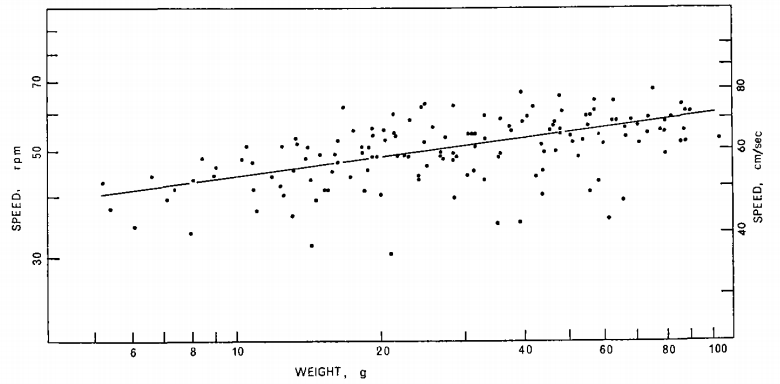
\includegraphics[width=1\textwidth]{chapter5/grafica tamano y velocidad de nado trucha arcoiris.png}
	\caption{Aproximación lineal de la relación entre peso y la velocidad de nado de truchas arcoíris}
	\begin{myflushleftportland}
		Fuente: \cite{Fry1970}
	\end{myflushleftportland}
	\label{fig:grafica tamano y velocidad de nado trucha arcoiris}
\end{myfigure}


En la Ecuación \ref{eq:ecuacion relacion tamano y velocidad de nado de trucha arcoiris} se muestra la relación entre \textit{X: peso de la trucha ($g$)} e \textit{Y: velocidad de nado ($cm/s$)} con un error \textit{Z= $\pm 0.033$}. 

\begin{myequation} \label{eq:ecuacion relacion tamano y velocidad de nado de trucha arcoiris}
	Y=-3.965+2.908(Z)X
\end{myequation}

En el caso de este trabajo, la dimensión máxima y mínima de las truchas arcoíris son de 20 cm y 15 cm, respectivamente. De la Tabla \ref{tbl:clasificacion de truchas por etapas de produccion} podemos obtener los gramos mediante interpolación lineal para cada límite: valores mínimo-máximo son 153 y 199 \textit{$g$}, respectivamente. Utilizando los valores antes indicados y empleando la Ecuación \ref{eq:ecuacion relacion tamano y velocidad de nado de trucha arcoiris} obtenemos los valores límites dentro del rango $[10.71; 15.13] (cm/s)$. Luego de escoger la máxima velocidad con redondeo hacia arriba (16 $cm/s$), ...


%% NUEVO SUBSECCION X.X.X.X
\subsubsection{Selección de indicadores}

Los indicadores ya sean visuales o sonoros son parte fundamental de una máquina. En el caso de la CCT\footnote{Máquina Contadora y Clasificadora de Truchas.} el sistema debe indicar al operario diversos estados o funciones: al detectar una trucha, al contar una trucha, al encender y al apagar.

\begin{itemize}
	\item \textbf{Indicador visual:} Lorem ipsum dolor sit amet, consectetur adipiscing elit, sed do eiusmod tempor incididunt ut labore et dolore magna aliqua. Lacus sed turpis tincidunt id aliquet. Vitae et leo duis ut diam. Dolor sit amet consectetur adipiscing elit ut aliquam purus sit. Dolor sed viverra ipsum nunc aliquet bibendum.
	
	\item \textbf{Indicador sonoro:} Una bocina indica al operario . En la Tabla \ref{tab:tabla comparativa de bocinas} se compara características técnicas entre algunas bocinas candidatas para el sistema.

	\begin{mytable}[H]
		\centering
		\caption{Tabla comparativa de bocinas}
		\label{tab:tabla comparativa de bocinas}
		\begin{tabular}{l|c|c|c|c|}
			\cline{2-5}
			\multicolumn{1}{c|}{\textbf{}}                         & \textbf{\begin{tabular}[c]{@{}c@{}}Requisitos\\ mínimos\end{tabular}} & \textbf{SE-B40} & \textbf{KH} & \textbf{TS-G1010F} \\ \hline
			\multicolumn{1}{|l|}{\textbf{Figura}}&
			-
			&
			\begin{minipage}{\mythirdmaxsizeofcontenttable}
				\centering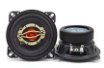
\includegraphics[width=\mythirdmaxsizeimageinsidetable]{chapter5/tablas comparativas/bocina 1.png} \\ 
				%\begin{myflushcenter}
				%	{\footnotesize Nombre imagen}
				%\end{myflushcenter}
			\end{minipage}  
			&
			\begin{minipage}{\mythirdmaxsizeofcontenttable}
				\centering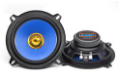
\includegraphics[width=\mythirdmaxsizeimageinsidetable]{chapter5/tablas comparativas/bocina 2.png} \\ 
				%\begin{myflushcenter}
				%	{\footnotesize Nombre imagen}
				%\end{myflushcenter}
			\end{minipage}
			&  
			\begin{minipage}{\mythirdmaxsizeofcontenttable}
				\centering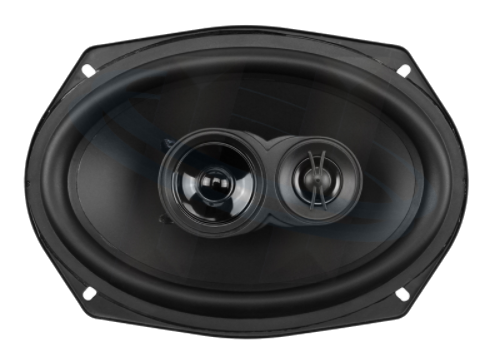
\includegraphics[width=\mythirdmaxsizeimageinsidetable]{chapter5/tablas comparativas/bocina 3.png} \\ 
				%\begin{myflushcenter}
				%	{\footnotesize Nombre imagen}
				%\end{myflushcenter}
			\end{minipage}  \\ \hline
			\multicolumn{1}{|l|}{\textbf{Fabricante}}              & -                                                                     &                 &             &                    \\ \hline
			\multicolumn{1}{|l|}{\textbf{Dimensión (cm.)}}         & -                                                                     &                 &             &                    \\ \hline
			\multicolumn{1}{|l|}{				
				\begin{minipage}{\myforthmaxsizeofcontenttable}	
					\textbf{Frecuencia de trabajo (Hz)}
				\end{minipage}
			}   & -                                                                     &                 &             &                    \\ \hline
			\multicolumn{1}{|l|}{
				\begin{minipage}{\myforthmaxsizeofcontenttable}	
					\textbf{Voltaje de alimentación (V)}
				\end{minipage}
			} & -                                                                     & 12 VDC          & 12 VDC      & 12 VDC             \\ \hline
			\multicolumn{1}{|l|}{\textbf{RMS (W)}}                 & -                                                                     & 80              & 25          & 30                 \\ \hline
			\multicolumn{1}{|l|}{\textbf{Precio (S/)}}             & -                                                                     & 105             & 105         & 79                 \\ \hline
			\multicolumn{1}{|l|}{\textbf{Disponibilidad}}          & Inmediata                                                             & A pedido        & A pedido    & A pedido           \\ \hline
		\end{tabular}
		\begin{flushleft}	
			Fuente: Imágenes de dominio público y elaboración propia.
		\end{flushleft}
	\end{mytable}

	[BORRADOR] El actuador lineal modelo XXX cumple con los requerimientos de la velocidad de movimiento que no puede ser demasiado lenta porque automatizar el proceso no sería óptimo, por lo que al final terminamos optando por el que tiene menor costo. [/BORRADOR]
	
\end{itemize}



%% NUEVO SUBSECCION X.X.X.X
\subsubsection{Selección de interruptor de seguridad de apagado de emergencia}

La implementación de un interruptor de seguridad es muy importante en el diseño de máquinas ya que es el mecanismo físico por el cual podemos parar la máquina quitando el suministro eléctrico a todos los componentes. En la Tabla \ref{tab:tabla comparativa de interruptor de seguridad de apagado de emergencia} se compara características técnicas entre interruptor de seguridad candidatos para el sistema.

\begin{mytable}[H]
	\centering
	\caption{Tabla comparativa de interruptor de seguridad de apagado de emergencia.}
	\label{tab:tabla comparativa de interruptor de seguridad de apagado de emergencia}
	\begin{tabular}{l|c|c|c|c|}
		\cline{2-5}
		\multicolumn{1}{c|}{\textbf{}}                          & \textbf{\begin{tabular}[c]{@{}c@{}}Requisitos\\ mínimos\end{tabular}} & \textbf{1} & \textbf{2} & \textbf{3} \\ \hline
		\multicolumn{1}{|l|}{\textbf{Figura}}&
		-
		&
		\begin{minipage}{\mythirdmaxsizeofcontenttable}
			\centering
\includegraphics[width=\mythirdmaxsizeimageinsidetable]{chapter5/tablas comparativas/interruptor de seguridad de apagado de emergencia 1.png} \\ 
			%\begin{myflushcenter}
			%	{\footnotesize Nombre imagen}
			%\end{myflushcenter}
		\end{minipage}  
		&
		\begin{minipage}{\mythirdmaxsizeofcontenttable}
			\centering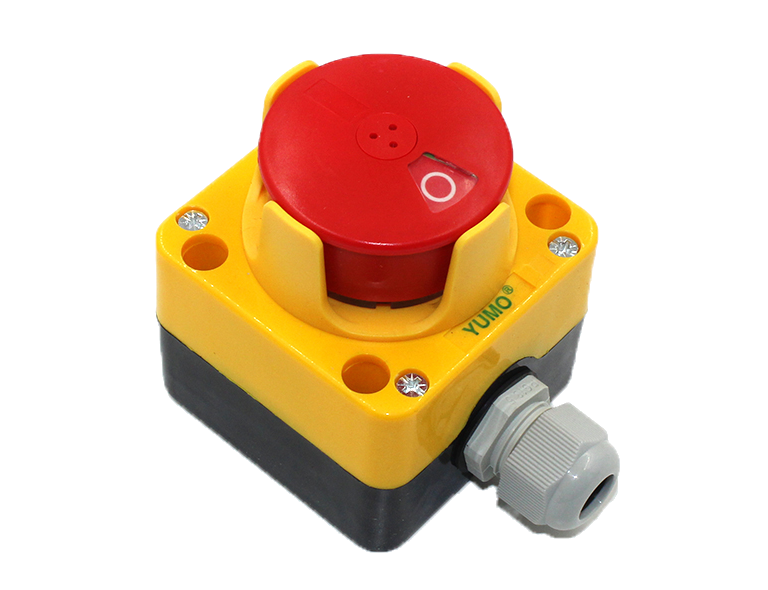
\includegraphics[width=\mythirdmaxsizeimageinsidetable]{chapter5/tablas comparativas/interruptor de seguridad de apagado de emergencia 2.png} \\ 
			%\begin{myflushcenter}
			%	{\footnotesize Nombre imagen}
			%\end{myflushcenter}
		\end{minipage}
		&  
		\begin{minipage}{\mythirdmaxsizeofcontenttable}
			\centering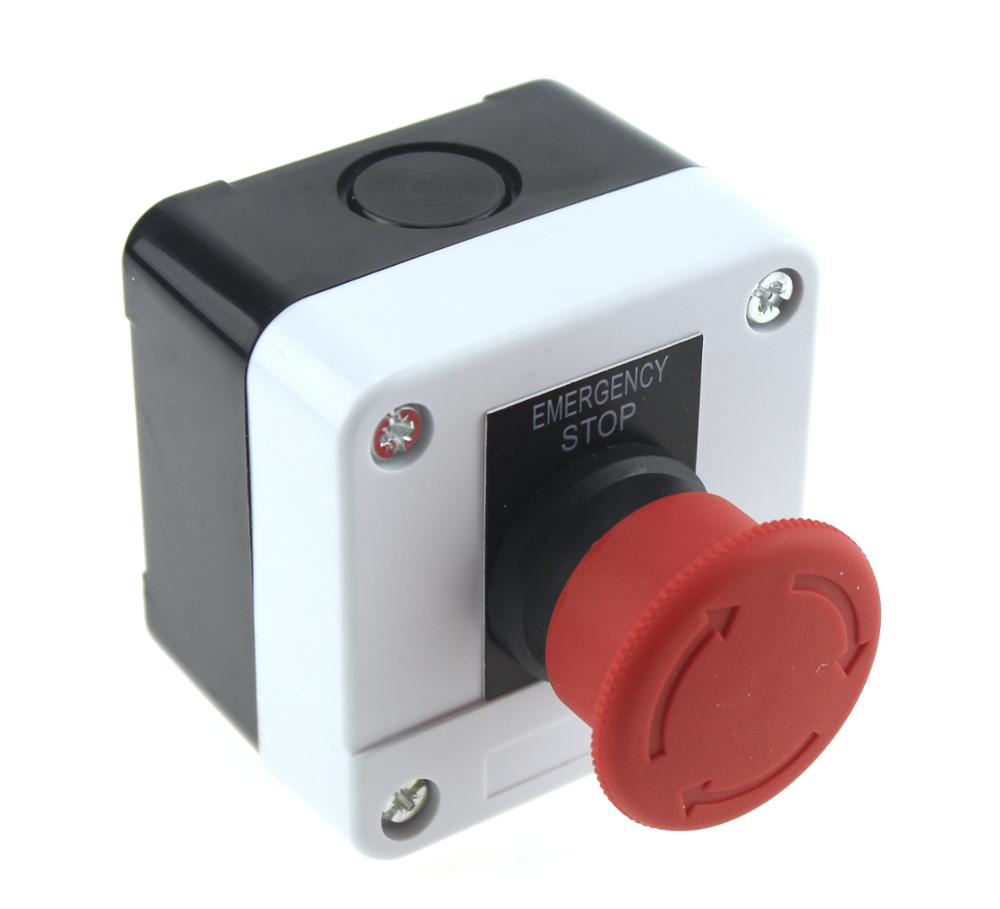
\includegraphics[width=\mythirdmaxsizeimageinsidetable]{chapter5/tablas comparativas/interruptor de seguridad de apagado de emergencia 3.png} \\ 
			%\begin{myflushcenter}
			%	{\footnotesize Nombre imagen}
			%\end{myflushcenter}
		\end{minipage}  \\ \hline
		\multicolumn{1}{|l|}{\textbf{Fabricante}}               & -                                                                     & 9          & 10         & 11         \\ \hline
		\multicolumn{1}{|l|}{\textbf{Nivel de protección}}      & 12                                                                    & 13         & 14         & 15         \\ \hline
		\multicolumn{1}{|l|}{
			\begin{minipage}{\myforthmaxsizeofcontenttable}			
				\textbf{Máximo voltaje admisible (V)}
			\end{minipage}
		}
		&
		16
		& 17         & 18         & 19         \\ \hline
		\multicolumn{1}{|l|}{
			\begin{minipage}{\myforthmaxsizeofcontenttable}			
				\textbf{Diámetro del botón (mm.)}
			\end{minipage}
		} & 20                                                                    & 21         & 22         & 23         \\ \hline
		\multicolumn{1}{|l|}{\textbf{Precio (S/)}}              & 24                                                                    & 25         & 26         & 27         \\ \hline
		\multicolumn{1}{|l|}{\textbf{Disponibilidad}}           & 32                                                                    & 33         & 34         & 35         \\ \hline
	\end{tabular}
	\begin{flushleft}	
		Fuente: Imágenes de dominio público y elaboración propia.
	\end{flushleft}
\end{mytable}

[BORRADOR] El actuador lineal modelo XXX cumple con los requerimientos de la velocidad de movimiento que no puede ser demasiado lenta porque automatizar el proceso no sería óptimo, por lo que al final terminamos optando por el que tiene menor costo. [/BORRADOR]


%% NUEVO SUBSECCION X.X.X.X
\subsubsection{Selección de interruptor de interruptor tipo hongo}

El encendido o apagado de la máquina es realizado por este interruptor, es decir, el control del suministro de energía del sistema depende de dicho dispositivo. En la Tabla \ref{tab:tabla comparativa de interruptor de interruptor tipo hongo} se compara características técnicas entre interruptores tipo hongo candidatos para el sistema.

\begin{mytable}[H]
\centering
\caption{Tabla comparativa de interruptor de interruptor tipo hongo.}
\label{tab:tabla comparativa de interruptor de interruptor tipo hongo}
\begin{tabular}{l|c|c|c|c|}
	\cline{2-5}
	\multicolumn{1}{c|}{\textbf{}}                          & \textbf{\begin{tabular}[c]{@{}c@{}}Requisitos\\ mínimos\end{tabular}} & \textbf{1} & \textbf{2} & \textbf{3} \\ \hline
	\multicolumn{1}{|l|}{\textbf{Figura}}&
	-
	&
	\begin{minipage}{\mythirdmaxsizeofcontenttable}
		\centering\includegraphics[width=\mythirdmaxsizeimageinsidetable]{chapter5/tablas comparativas/interruptor tipo hongo 1.png} \\ 
		%\begin{myflushcenter}
		%	{\footnotesize Nombre imagen}
		%\end{myflushcenter}
	\end{minipage}  
	&
	\begin{minipage}{\mythirdmaxsizeofcontenttable}
		\centering\includegraphics[width=\mythirdmaxsizeimageinsidetable]{chapter5/tablas comparativas/interruptor tipo hongo 2.png} \\ 
		%\begin{myflushcenter}
		%	{\footnotesize Nombre imagen}
		%\end{myflushcenter}
	\end{minipage}
	&  
	\begin{minipage}{\mythirdmaxsizeofcontenttable}
		\centering\includegraphics[width=\mythirdmaxsizeimageinsidetable]{chapter5/tablas comparativas/interruptor tipo hongo 3.png} \\ 
		%\begin{myflushcenter}
		%	{\footnotesize Nombre imagen}
		%\end{myflushcenter}
	\end{minipage}  \\ \hline
	\multicolumn{1}{|l|}{\textbf{Fabricante}}               & -                                                                     & 9          & 10         & 11         \\ \hline
	\multicolumn{1}{|l|}{\textbf{Nivel de protección}}      & 12                                                                    & 13         & 14         & 15         \\ \hline
	\multicolumn{1}{|l|}{
		\begin{minipage}{\myforthmaxsizeofcontenttable}			
			\textbf{Máximo voltaje admisible (V)}
		\end{minipage}
	}
	&
	16
	& 17         & 18         & 19         \\ \hline
	\multicolumn{1}{|l|}{
			\begin{minipage}{\myforthmaxsizeofcontenttable}			
				\textbf{Diámetro del botón (mm.)}
			\end{minipage}
	} & 20                                                                    & 21         & 22         & 23         \\ \hline
	\multicolumn{1}{|l|}{\textbf{Precio (S/)}}              & 24                                                                    & 25         & 26         & 27         \\ \hline
	\multicolumn{1}{|l|}{\textbf{Disponibilidad}}           & 32                                                                    & 33         & 34         & 35         \\ \hline
	\end{tabular}
	\begin{flushleft}	
		Fuente: Imágenes de dominio público y elaboración propia.
	\end{flushleft}
\end{mytable}

[BORRADOR] El actuador lineal modelo XXX cumple con los requerimientos de la velocidad de movimiento que no puede ser demasiado lenta porque automatizar el proceso no sería óptimo, por lo que al final terminamos optando por el que tiene menor costo. [/BORRADOR]

%% NUEVO SUBSECCION X.X.X.X
\subsubsection{Cálculo del consumo de energía del sistema} 

El cálculo del consumo de energía del sistema es la suma de potencia requerida por cada componente. Dicha información se presenta en la Tabla \ref{fig:potencia requerida por componente}, además se muestra el modelo, la potencia máxima, voltaje de cada componente. Se considera, también, la cantidad de cada modelo de componente electrónico usado en el sistema.

% TIENE QUE SER TABLA
% TIENE QUE SER TABLA
% TIENE QUE SER TABLA
% TIENE QUE SER TABLA
% TIENE QUE SER TABLA
     
\begin{myfigure}[H]
	\centering
	\includegraphics[width=1\textwidth]{chapter5/potencia requerida por componente.png}
	\caption{Potencia requerida por componente}
	\begin{myflushleftportland}
		Fuente: Elaboración propia.
	\end{myflushleftportland}
	\label{fig:potencia requerida por componente}
\end{myfigure}


%% NUEVO SUBSECCION X.X.X.X
\subsubsection{Diagrama de flujo}

El diagrama de flujo principal, expuesto en la Figura \ref{fig:diagrama de flujo} describe los pasos necesarios para el control del sistema. .. ... .. [Explicar diagrama de flujo]

\begin{myfigure}[H]
	\centering
	\includegraphics[width=1\textwidth]{chapter5/diagrama de flujo.png}
	\caption{Diagrama de flujo principal}
	\begin{myflushleftportland}
		Fuente: Elaboración propia.
	\end{myflushleftportland}
	\label{fig:diagrama de flujo}
\end{myfigure}


%% NUEVO SUBSECCION X.X.X.X
\subsubsection{Diseño frontend de la aplicación móvil}

La aplicación móvil permitirá a un operario visualizar los estados de la máquina, así como tener un registro de la clasificación y conteo de truchas, es decir, extraer los datos luego de ser procesados por la máquina CCT de manera inalámbrica al terminar el proceso. Además, posterior a este trabajo, podría agregarse más características al aplicativo móvil. El framework de desarrollo del aplicativo, que no se desarrollará en el presente trabajo, escogido es Flutter por su paradigma multiplataforma, es decir, escribir un programa que se vea igual en los sistemas operativos Android y iOS \cite{Simone2020}. El diseño frontend escogido para el proyecto y su desarrollo sencillo 

Designing the obvious
\cite{Joekman2010} \\
Google Flutter Mobile Development Quick Start Guide
\cite{PrajyotMainkar2019} \\
Mobile Learning Design: Theories and Application
\cite{Churchill2016} \\
Mobile Design Pattern Gallery: UI Patterns for Mobile Applications
\cite{Neil2012}


\begin{myfigure}[H]
	\centering
	\includegraphics[width=1\textwidth]{chapter5/aplicacion movil login.png}
	\caption{Aplicación móvil: inicio de sesión}
	\begin{myflushleftportland}
		Fuente: Elaboración propia.
	\end{myflushleftportland}
	\label{fig:aplicacion movil login}
\end{myfigure}


%% NUEVA SECCIÓN X.X.X
\subsection{Subsistema de flotación}
\label{ssec:subsistema de flotacion}

Luego de definir en las Secciones \ref{ssec:subsistema de recepcion y traslado de truchas}, \ref{ssec:subsistema de procesamiento de imágenes}, \ref{ssec:subsistema de suministro de energia}, y \ref{ssec:subsistema de control e interaccion con el usuario}, la selección de los dispositivos y su interacción el sistema permiten calcular las dimensiones de la máquina para analizar la flotabilidad y seleccionar flotadores adecuados. En las siguientes subsecciones se analizan los cálculos, selección y diseño del sistema de flotación.

%% NUEVO SUBSECCION X.X.X.X
\subsubsection{Cálculo de sistema flotador}

Lacus sed turpis tincidunt id aliquet. Nunc aliquet bibendum enim facilisis gravida neque convallis a. Ut tellus elementum sagittis vitae et leo duis ut diam. Dolor sit amet consectetur adipiscing elit ut aliquam purus sit. 

%% NUEVO SUBSECCION X.X.X.X
\subsubsection{Selección de flotadores}

Lacus sed turpis tincidunt id aliquet. Nunc aliquet bibendum enim facilisis gravida neque convallis a. Ut tellus elementum sagittis vitae et leo duis ut diam. Dolor sit amet consectetur adipiscing elit ut aliquam purus sit. 


\begin{mytable}[H]
	\centering
	\caption{Tabla comparativa de flotadores.}
	\label{tab:tabla comparativa de flotadores}
	\begin{tabular}{l|c|c|c|c|}
		\cline{2-5}
		\multicolumn{1}{c|}{\textbf{}}                          & \textbf{\begin{tabular}[c]{@{}c@{}}Requisitos\\ mínimos\end{tabular}} & \textbf{1} & \textbf{2} & \textbf{3} \\ \hline
		\multicolumn{1}{|l|}{\textbf{Figura}}&
		-
		&
		\begin{minipage}{\mythirdmaxsizeofcontenttable}
			\centering\includegraphics[width=\mythirdmaxsizeimageinsidetable]{chapter5/tablas comparativas/flotador 1.png} \\ 
			%\begin{myflushcenter}
			%	{\footnotesize Nombre imagen}
			%\end{myflushcenter}
		\end{minipage}  
		&
		\begin{minipage}{\mythirdmaxsizeofcontenttable}
			\centering\includegraphics[width=\mythirdmaxsizeimageinsidetable]{chapter5/tablas comparativas/flotador 2.png} \\ 
			%\begin{myflushcenter}
			%	{\footnotesize Nombre imagen}
			%\end{myflushcenter}
		\end{minipage}
		&  
		\begin{minipage}{\mythirdmaxsizeofcontenttable}
			\centering\includegraphics[width=\mythirdmaxsizeimageinsidetable]{chapter5/tablas comparativas/flotador 3.png} \\ 
			%\begin{myflushcenter}
			%	{\footnotesize Nombre imagen}
			%\end{myflushcenter}
		\end{minipage}  \\ \hline
		\multicolumn{1}{|l|}{\textbf{Fabricante}}               & -                                                                     & 9          & 10         & 11         \\ \hline
		\multicolumn{1}{|l|}{\textbf{Característica}}      & 12                                                                    & 13         & 14         & 15         \\ \hline
		\multicolumn{1}{|l|}{
			\begin{minipage}{\myforthmaxsizeofcontenttable}			
				\textbf{Característica}
			\end{minipage}
		}
		&
		16
		& 17         & 18         & 19         \\ \hline
		\multicolumn{1}{|l|}{
			\begin{minipage}{\myforthmaxsizeofcontenttable}			
				\textbf{Característica}
			\end{minipage}
		} & 20                                                                    & 21         & 22         & 23         \\ \hline
		\multicolumn{1}{|l|}{\textbf{Característica}}              & 24                                                                    & 25         & 26         & 27         \\ \hline
		\multicolumn{1}{|l|}{\textbf{Característica}}           & 32                                                                    & 33         & 34         & 35         \\ \hline
	\end{tabular}
	\begin{flushleft}	
		Fuente: Imágenes de dominio público y elaboración propia.
	\end{flushleft}
\end{mytable}

[BORRADOR] El actuador lineal modelo XXX cumple con los requerimientos de la velocidad de movimiento que no puede ser demasiado lenta porque automatizar el proceso no sería óptimo, por lo que al final terminamos optando por el que tiene menor costo. [/BORRADOR]

%% NUEVO SUBSECCION X.X.X.X
\subsubsection{Diseño de sistema de flotación}

Lacus sed turpis tincidunt id aliquet. Nunc aliquet bibendum enim facilisis gravida neque convallis a. Ut tellus elementum sagittis vitae et leo duis ut diam. Dolor sit amet consectetur adipiscing elit ut aliquam purus sit. 



%% NUEVA SECCIÓN X.X.X
\subsection{Planos del sistema}
\label{ssec:planos del sistema}

Los planos permiten visualizar el sistema de una forma en particular dependiendo del tipo de plano. En el presente trabajo optaremos por incluir dos tipos: planos de ensamble y planos de despiece.

%% NUEVO SUBSECCION X.X.X.X
\subsubsection{Lista de planos de ensamble}

El plano de ensamble presenta una visión de los diferentes componentes, cómo son las juntas, incluye un listado de componentes y se proporcionan características técnicas como el  tipo de material y cantidad de componentes similares.\footnote{\cite{Goetsch2010}} En la Tabla \ref{tab:lista de planos de ensamble} se muestra una lista de planos de ensamble.


\begin{mytable}[H]
	\centering
	\caption{Lista de planos de ensamble.}
	\label{tab:lista de planos de ensamble}
	\begin{tabular}{|c|c|c|}
		\hline
		\textbf{N° Lámina} & \textbf{Plano} & \textbf{Tamaño de pieza} \\ \hline
		\textbf{L1}        & 1              & 2             \\ \hline
		\textbf{L2}        & 3              & 4             \\ \hline
		\textbf{L3}        & 5              & 6             \\ \hline
		\textbf{L4}        & 7              & 8             \\ \hline
		\textbf{L5}        & 9              & 10            \\ \hline
		\textbf{L6}        & 11             & 12            \\ \hline
		\textbf{L7}        & 13             & 14            \\ \hline
	\end{tabular}
	\begin{flushleft}	
	Fuente: Elaboración propia.
\end{flushleft}
\end{mytable}


%% NUEVO SUBSECCION X.X.X.X
\subsubsection{Plano de despiece}

El plano de despiece presenta las características técnicas de cada pieza. Muestra dimensiones para poder fabricar la pieza. En la Tabla \ref{tab:plano de despiece} se muestra una lista de planos de despiece de cada pieza.

\begin{mytable}[H]
	\centering
	\caption{Lista de planos de despiece}
	\label{tab:plano de despiece}
	\begin{tabular}{|c|c|c|}
		\hline
		\textbf{N°} & \textbf{Nombre de pieza} & \textbf{Tamaño de página} \\ \hline
		\textbf{1}  & 1                        & 2                         \\ \hline
		\textbf{2}  & 3                        & 4                         \\ \hline
		\textbf{3}  & 5                        & 6                         \\ \hline
		\textbf{4}  & 7                        & 8                         \\ \hline
		\textbf{5}  & 9                        & 10                        \\ \hline
		\textbf{6}  & 11                       & 12                        \\ \hline
		\textbf{7}  & 13                       & 14                        \\ \hline
	\end{tabular}
	\begin{flushleft}	
	Fuente: Elaboración propia.
\end{flushleft}
\end{mytable}
